\documentclass[11pt,a4paper]{article}
\usepackage[T1]{fontenc}
\usepackage[utf8]{inputenc}
\usepackage{lmodern}
\usepackage[margin=2.4cm]{geometry}
\usepackage{amsmath,amssymb,amsthm,bm}
\usepackage{booktabs,tabularx,longtable,multirow,array}
\usepackage{graphicx,float,xcolor}
\usepackage{fancyhdr}
\usepackage{algorithm,algorithmic}
\usepackage{verbatim,url}
\usepackage{tikz}
\usetikzlibrary{arrows.meta,positioning,shapes.geometric,calc,fit,backgrounds,decorations.pathreplacing}
\usepackage[colorlinks=true,linkcolor=blue!50!black,citecolor=green!40!black,urlcolor=blue!60!black]{hyperref}

\newcommand{\ket}[1]{\left|#1\right\rangle}
\newcommand{\bra}[1]{\left\langle#1\right|}
\newcommand{\braket}[2]{\left\langle#1\middle|#2\right\rangle}
% \code{}: typewriter text in which every underscore is a permitted line break
\newcommand{\codeus}{\textunderscore\allowbreak}
\newcommand{\code}[1]{{\small\ttfamily\let\_\codeus #1}}
\emergencystretch=2.5em
\newcommand{\R}{\mathbb{R}}
\newtheorem{proposition}{Proposition}
\newtheorem{definition}{Definition}

\definecolor{qblue}{HTML}{2563EB}
\definecolor{qorange}{HTML}{EA580C}
\definecolor{qgreen}{HTML}{16A34A}
\definecolor{qgrey}{HTML}{6B7280}
\definecolor{boxbg}{HTML}{F1F5F9}

% simple shaded "key finding" box without extra packages
\newcommand{\keybox}[2]{%
  \par\medskip\noindent
  \colorbox{boxbg}{\parbox{\dimexpr\linewidth-2\fboxsep}{%
  \textbf{\color{qblue}#1}\par\smallskip #2}}\par\medskip}

\pagestyle{fancy}
\fancyhf{}
\fancyhead[L]{\small Quantum Kernel Network Intrusion Detection}
\fancyhead[R]{\small Improvement Report}
\fancyfoot[C]{\thepage}
\renewcommand{\headrulewidth}{0.4pt}
\setlength{\headheight}{14pt}
\setlength{\parskip}{4pt}
\renewcommand{\arraystretch}{1.15}

\begin{document}

\begin{titlepage}
\centering
\vspace*{2.5cm}
{\LARGE\bfseries Network Intrusion Detection with\\[4pt] Quantum Kernel Support Vector Machines\par}
\vspace{0.8cm}
{\Large Project Documentation and Improvement Report\par}
\vspace{0.4cm}
{\large CIC-DDoS2019 \textbullet{} ZZ Entangling Feature Map \textbullet{} Google Cirq\par}
\vspace{2cm}
\begin{minipage}{0.82\linewidth}
\small
This report explains the whole project in detail: the dataset, the classical and quantum
machine-learning theory behind it, and the original code and its results. It then documents
every improvement made to the code and why, with derivations and verification, and reports a
complete re-evaluation under a leakage-free, statistically controlled protocol. Exact commands
to reproduce every result are given in \code{TESTING.md} and Appendix~\ref{app:commands}.
\end{minipage}
\vfill
{\large Department of Computer Engineering\par}
\vspace{0.3cm}
{\normalsize \today\par}
\end{titlepage}

\begin{abstract}
\noindent
The project classifies network flows from the CIC-DDoS2019 benchmark as benign or as one of
five DDoS attack types. It uses a quantum support vector machine (QSVM) whose kernel is the
fidelity between quantum states prepared by a ZZ entangling feature map, simulated with
Google Cirq. The original implementation reported that the entangled kernel beats a classical
RBF-SVM by +1.8 points (binary) and +12 points (6-class). We audited the code and data and
found five issues that affect those conclusions: (i)~65\% of the rows in the data file are exact
duplicates, so about 30\% of test flows have an identical copy in the training set; (ii)~a
min--max scaler was fitted on the whole dataset before the train/test split; (iii)~heavy-tailed
flow features were mapped linearly onto rotation angles, which wastes most of the angle range;
(iv)~neither the quantum kernel's bandwidth nor the SVM hyperparameters were tuned, and the
classical baseline was never tuned at all; (v)~each kernel entry simulated two full circuits,
so a $1600\times1600$ kernel at 16 qubits cost an estimated 44 hours.

We kept the project's architecture and fixed each issue: deduplication, train-only
preprocessing with a signed log transform, a bandwidth parameter $\alpha$ tuned by
cross-validation together with $C$ (and $C,\gamma$ for the RBF baseline), and an exact
NumPy statevector engine that uses the diagonal structure of the ZZ map. The engine matches
Cirq to $10^{-7}$, simulates each sample once instead of twice per kernel entry, and computes
the same 16-qubit kernels in about 26 seconds. We also added macro-F1, MCC, false-alarm and
detection rates, multi-seed confidence intervals, McNemar significance tests, kernel-concentration
and kernel--target-alignment diagnostics, the geometric-difference test of Huang et al., a
Random-Forest reference, unit tests and a resumable benchmark suite.

Under the corrected protocol, all models reach high accuracy, and the quantum kernel performs
on par with a tuned classical kernel on the same features. The large advantages reported earlier
come mainly from the leakage and from the untuned baseline, not from entanglement. The
diagnostics explain why, and they show where a quantum kernel could still help.
\end{abstract}

\clearpage
\tableofcontents
\clearpage

\section{Introduction}
\label{sec:intro}

\subsection{Motivation}
Distributed Denial-of-Service (DDoS) attacks overwhelm a target with traffic from many sources.
They remain among the most frequent and most costly attacks on networked infrastructure. Modern
DDoS campaigns often use \emph{reflection and amplification}: the attacker sends small requests
with a spoofed source address to public servers (LDAP, MSSQL, Portmap/rpcbind, and so on), and
those servers send much larger responses to the victim. Signature-based detection struggles
against these attacks because the packets are individually legitimate. Detection therefore
relies on statistical features of whole \emph{flows}: packet counts, sizes, inter-arrival times,
TCP flags and rates. Those features are what machine-learning classifiers learn from.

Quantum machine learning (QML) asks whether quantum computers can help with such learning
problems. One of its most studied ideas is the \emph{quantum kernel method}. A classical
data point $\bm{x}$ is encoded into a quantum state $\ket{\phi(\bm{x})}$ in a Hilbert space of
dimension $2^n$. The overlap $K(\bm{x},\bm{x}')=|\braket{\phi(\bm{x})}{\phi(\bm{x}')}|^2$ is then
used as the kernel of an ordinary support vector machine. Havlíček et al.~\cite{havlicek2019}
proposed the \emph{ZZ feature map}, an entangling circuit whose kernel is believed to be hard to
evaluate classically for large $n$. That hardness is a prerequisite for a quantum advantage.

\subsection{The project}
This project applies quantum kernel SVMs (QSVMs) to network intrusion detection on the
CIC-DDoS2019 dataset~\cite{sharafaldin2019ddos}. The accompanying paper~\cite{ourpaper} compares three methods:
\begin{enumerate}
  \item an \textbf{Analytical kernel} built from single-qubit $R_x$ rotations. This is a separable
        product state, so its kernel has the closed form $\prod_i\cos^2((b_i-a_i)/2)$;
  \item a \textbf{Sampling kernel}, which estimates the same overlaps by running the circuit
        $U^\dagger(\bm{a})U(\bm{b})$ for 1024 shots, as real hardware would;
  \item a \textbf{ZZ entangling kernel}, which uses the Havlíček feature map and exact statevector simulation.
\end{enumerate}
All three are compared with a classical RBF-kernel SVM. The paper reports that the ZZ kernel wins
in both settings: 98.79\% vs.\ 96.97\% in binary classification (benign vs.\ DDoS) and
92.00\% vs.\ 80.00\% in 6-class classification. It concludes that entanglement is necessary for a
quantum advantage on this task.

\subsection{Goal of this report}
The task was to \emph{build on the current state of the project}: improve the existing code
without replacing it with something unrelated, then document the whole project and every change.
The improved code keeps the same three modules (\code{data\_loader.py}, \code{qsvm.py},
\code{main.py}), the same Cirq ZZ feature map class, the same CLI flags and the same dataset. We
added two small modules (\code{preprocessing.py}, \code{evaluation.py}) and three supporting
tools (\code{benchmark.py}, \code{make\_figures.py}, \code{tests/}). The original code is preserved
unchanged in \code{legacy/}, and \code{main.py --legacy} reproduces its protocol exactly.

The report has three parts:
\begin{itemize}
  \item \textbf{Part I: the project as it was} (Sections~\ref{sec:background}--\ref{sec:original}).
        It covers the background theory (DDoS, SVMs, quantum computing, quantum kernels), the
        dataset as it actually exists in this repository, and a walk-through and audit of the
        original pipeline.
  \item \textbf{Part II: the improvements} (Sections~\ref{sec:impdata}--\ref{sec:evalsw}).
        They are grouped into data integrity, computation, modelling, and evaluation/software.
        Each one comes with its motivation, the change, a derivation where needed, and how it was
        verified.
  \item \textbf{Part III: results and discussion} (Sections~\ref{sec:results}--\ref{sec:discussion}).
        This part re-runs the paper's comparison under the corrected protocol with 5 random seeds,
        adds ablations isolating each fix, and runs sweeps over bandwidth, qubit count, shots,
        circuit architecture, feature set and training-set size. It then discusses what the
        evidence says about quantum advantage on this task.
\end{itemize}

\keybox{Summary of findings}{%
\begin{itemize}\itemsep0pt
\item The data file contains 49{,}393 exact duplicate rows (65.9\%). With duplicates kept, about
      30\% of test flows have an identical twin in the training set.
\item The original kernel computation is exact but needed $2N^2$ circuit simulations. The new
      engine needs $N$ and gives the same numbers to $10^{-7}$, with speed-ups of $10^3$--$10^5\times$
      (Table~\ref{tab:speed}).
\item With 16 qubits and the original angle scale, the ZZ kernel is \emph{concentrated}: the median
      off-diagonal entry is $\approx2\times10^{-5}$ and the kernel matrix is close to the identity. A tuned bandwidth
      $\alpha<1$ fixes this.
\item Once the classical baseline gets the same preprocessing and the same tuning budget, the
      large QSVM advantages disappear. Section~\ref{sec:results} gives the numbers.
\end{itemize}}

\section{Background}
\label{sec:background}

\subsection{DDoS attacks in the dataset}
CIC-DDoS2019 groups attacks into \emph{reflection-based} attacks, where third-party servers
answer spoofed requests and so hide and amplify the attacker, and \emph{exploitation-based}
attacks, which abuse protocol behaviour directly~\cite{sharafaldin2019ddos}. The five attack
classes in this project's data file are summarised in Table~\ref{tab:attacks}.

\begin{table}[H]
\centering\small
\caption{Attack classes present in \code{output.csv}.}
\label{tab:attacks}
\begin{tabularx}{\linewidth}{l l X}
\toprule
Label & Type & Mechanism \\
\midrule
\code{MSSQL} & reflection (TCP/UDP) & Spoofed requests to the SQL Server Resolution Protocol
  (UDP 1434). Servers answer with much larger instance listings. \\
\code{LDAP} & reflection (UDP) & Connectionless LDAP (CLDAP, UDP 389) queries whose responses are
  tens of times larger than the request. \\
\code{Portmap} & reflection (UDP) & Abuse of the RPC port mapper (rpcbind, UDP 111), which returns
  long service lists. \\
\code{UDP} & exploitation & High-rate flood of UDP datagrams to random ports. The victim spends
  resources answering with ICMP ``port unreachable''. \\
\code{Syn} & exploitation (TCP) & SYN flood: many half-open TCP handshakes exhaust the victim's
  connection table. \\
\code{BENIGN} & --- & Normal background traffic generated by profiled user agents. \\
\bottomrule
\end{tabularx}
\end{table}

These classes leave different traces at the flow level. SYN floods produce very short flows with
the SYN flag set and almost no backward traffic. Reflection attacks produce unidirectional flows
with characteristic payload sizes. Benign traffic is far more varied. This is why flow statistics
separate benign from attack traffic so well, and also why the \emph{reflection} classes (MSSQL,
LDAP, Portmap) are the hard part of the multiclass problem: they look alike.

\subsection{Flow-based detection and CICFlowMeter}
A \emph{flow} is the set of packets sharing a 5-tuple (source/destination IP and port, protocol)
within a timeout. CICFlowMeter~\cite{sharafaldin2018} turns packet captures into bidirectional
flows and computes about 80 statistics per flow: durations, forward/backward packet counts and
byte totals, packet-length moments, inter-arrival-time (IAT) moments, TCP flag counts, header
lengths, bulk and sub-flow statistics, and active/idle periods. Two properties of these features
matter a great deal later:
\begin{itemize}
\item \textbf{Heavy tails.} Rates such as \code{Flow Bytes/s} span nine orders of magnitude
      (Section~\ref{sec:dataset}).
\item \textbf{Redundancy.} Many columns are deterministic functions of others (e.g.\
      \code{Fwd Header Length.1} duplicates \code{Fwd Header Length}; \code{Packet Length Variance}
      is the square of \code{Packet Length Std}), and several are always zero.
\end{itemize}

\subsection{Support vector machines and kernels}
Given training data $\{(\bm{x}_i,y_i)\}_{i=1}^N$ with $y_i\in\{-1,+1\}$, a soft-margin SVM~\cite{cortes1995}
solves the dual problem
\begin{equation}
\max_{\bm{\beta}}\;\sum_{i}\beta_i-\frac12\sum_{i,j}\beta_i\beta_j y_iy_j K(\bm{x}_i,\bm{x}_j)
\quad\text{s.t.}\quad 0\le\beta_i\le C,\;\; \sum_i\beta_iy_i=0,
\label{eq:svmdual}
\end{equation}
and predicts $f(\bm{x})=\operatorname{sign}\big(\sum_i\beta_iy_iK(\bm{x}_i,\bm{x})+b\big)$.
The data enter \emph{only} through the kernel $K(\bm{x},\bm{x}')=\langle\varphi(\bm{x}),\varphi(\bm{x}')\rangle$,
the inner product in some feature space. This is the \emph{kernel trick}: any positive
semi-definite (PSD) function can be plugged in, including one evaluated on a quantum computer.
scikit-learn's \code{SVC(kernel='precomputed')} accepts the $N\times N$ Gram matrix
$K_{ij}=K(\bm{x}_i,\bm{x}_j)$ for training and the $M\times N$ matrix
$K(\bm{x}^{\text{test}}_m,\bm{x}_i)$ for prediction~\cite{sklearn}.

\paragraph{The RBF kernel.} The classical baseline is $K_{\text{RBF}}(\bm{x},\bm{x}')=\exp(-\gamma\|\bm{x}-\bm{x}'\|^2)$.
The \emph{bandwidth} $\gamma$ sets the scale at which two points count as similar. If $\gamma$ is
too large, $K\to I$ and the SVM memorises the training set. If it is too small, $K\to\bm{1}\bm{1}^\top$
and every point looks the same. This idea carries over directly to quantum kernels
(Section~\ref{sec:conc}).

\paragraph{Regularisation $C$.} $C$ trades margin width against training errors. $C$ and $\gamma$
interact strongly, which is why they are normally tuned jointly by cross-validation.

\paragraph{Multiclass and probabilities.} For $k$ classes, \code{SVC} trains $k(k-1)/2$
one-vs-one classifiers and takes a vote. Probabilities (\code{predict\_proba}) come from Platt
scaling~\cite{platt1999}, a logistic model fitted on internal cross-validation folds. Platt
scaling is randomised, so it must be seeded to be reproducible.

\subsection{Quantum computing essentials}
A qubit is a unit vector $\ket{\psi}=a\ket0+b\ket1\in\mathbb{C}^2$. An $n$-qubit register lives in
$(\mathbb{C}^2)^{\otimes n}\cong\mathbb{C}^{2^n}$, with basis states $\ket{z}$ indexed by bit-strings
$z\in\{0,1\}^n$. Gates are unitary matrices. The ones used here are
\begin{equation}
H=\tfrac{1}{\sqrt2}\begin{pmatrix}1&1\\1&-1\end{pmatrix},\quad
R_z(\theta)=\begin{pmatrix}e^{-i\theta/2}&0\\0&e^{i\theta/2}\end{pmatrix},\quad
R_x(\theta)=\begin{pmatrix}\cos\frac\theta2&-i\sin\frac\theta2\\-i\sin\frac\theta2&\cos\frac\theta2\end{pmatrix},
\end{equation}
and the two-qubit $\mathrm{CNOT}\ket{a,b}=\ket{a,a\oplus b}$. Measuring in the computational basis
returns $z$ with probability $|\braket{z}{\psi}|^2$ (the Born rule). A classical
\emph{statevector simulator} stores all $2^n$ complex amplitudes. With \code{complex64} this needs
$8\cdot2^n$ bytes: 2\,KB at 8 qubits, 512\,KB at 16 and 8\,MB at 20. A 58-qubit state would need
about 2.3 exabytes, which is why the features are first reduced with PCA. The paper's figure of
128\,GB for 58 qubits is a typo; $8\cdot 2^{58}$ bytes $\approx 2.3\times10^{18}$ bytes.

\paragraph{Useful identities.}
Writing $s(z)=1-2z\in\{+1,-1\}$ for the eigenvalue of $Z$ on bit $z$, we have
$R_z(\theta)\ket{z}=e^{-i\theta s(z)/2}\ket z$: $R_z$ is \emph{diagonal}. The sequence
$\mathrm{CNOT}_{ij}\,R_z^{(j)}(\theta)\,\mathrm{CNOT}_{ij}$ maps
$\ket{z_i,z_j}\mapsto e^{-i\theta s(z_i\oplus z_j)/2}\ket{z_i,z_j}$, and since $s(z_i\oplus z_j)=s(z_i)s(z_j)$,
\begin{equation}
\mathrm{CNOT}_{ij}\,R_z^{(j)}(\theta)\,\mathrm{CNOT}_{ij}=\exp\!\big(-i\tfrac{\theta}{2}Z_i Z_j\big),
\label{eq:zzgate}
\end{equation}
which is also diagonal. This is the ``ZZ interaction'' of the feature map, and it is the key to the
fast simulator in Section~\ref{sec:impcompute}.

\subsection{Quantum feature maps and kernels}
A \emph{feature map} is a parameterised circuit $U(\bm{x})$ that prepares $\ket{\phi(\bm x)}=U(\bm x)\ket{0^n}$.
The \emph{fidelity quantum kernel} is
\begin{equation}
K(\bm a,\bm b)=\big|\braket{\phi(\bm a)}{\phi(\bm b)}\big|^2=\big|\bra{0^n}U^\dagger(\bm a)U(\bm b)\ket{0^n}\big|^2 .
\label{eq:qkernel}
\end{equation}
The second form shows how hardware computes it: prepare $U^\dagger(\bm a)U(\bm b)\ket{0^n}$,
measure all qubits, and record how often the all-zeros string appears. $K$ is a valid PSD kernel,
because it is the inner product of the ``density-matrix features''
$\rho(\bm x)=\ket{\phi(\bm x)}\!\bra{\phi(\bm x)}$ under the Hilbert--Schmidt inner product~\cite{schuld2019,schuld2021}.
It also satisfies $K(\bm x,\bm x)=1$.

\paragraph{Separable $R_x$ encoding (Method 1).} With $\ket{\phi(\bm x)}=\bigotimes_i R_x(x_i)\ket0$,
the overlap factorises qubit by qubit. Since $R_x(a)^\dagger R_x(b)=R_x(b-a)$ and
$\bra0R_x(\theta)\ket0=\cos(\theta/2)$,
\begin{equation}
K_{R_x}(\bm a,\bm b)=\prod_{i=1}^n\cos^2\!\Big(\frac{b_i-a_i}{2}\Big).
\label{eq:rxkernel}
\end{equation}
This is a classical, cheap-to-evaluate kernel. It is a product of one-dimensional kernels, and
it closely resembles a periodic RBF kernel. No quantum computer is needed to evaluate it.

\paragraph{ZZ feature map (Method 3).} Following~\cite{havlicek2019}, one repetition is
\begin{equation}
U_{\text{ZZ}}(\bm x)=\underbrace{\prod_{(i,j)\in E}\exp\!\big(-i(\pi-x_i)(\pi-x_j)Z_iZ_j\big)\prod_i e^{-ix_iZ_i}}_{D(\bm x)\ \text{(diagonal)}}\;H^{\otimes n},
\label{eq:zzmap}
\end{equation}
where $E$ is the set of entangled pairs (adjacent pairs, \emph{linear}, in the original code) and
the whole block is repeated $r$ times. The code implements $e^{-ix_iZ_i}$ as $R_z(2x_i)$ and the
pair term as $\mathrm{CNOT}\cdot R_z(2(\pi-x_i)(\pi-x_j))\cdot\mathrm{CNOT}$, using
Eq.~\eqref{eq:zzgate}. Figure~\ref{fig:circuit} shows one repetition on four qubits. For $r\ge2$,
the Hadamard layers sandwiched between diagonal layers are what is conjectured to make the kernel
hard to compute classically~\cite{havlicek2019}.

\begin{figure}[H]
\centering
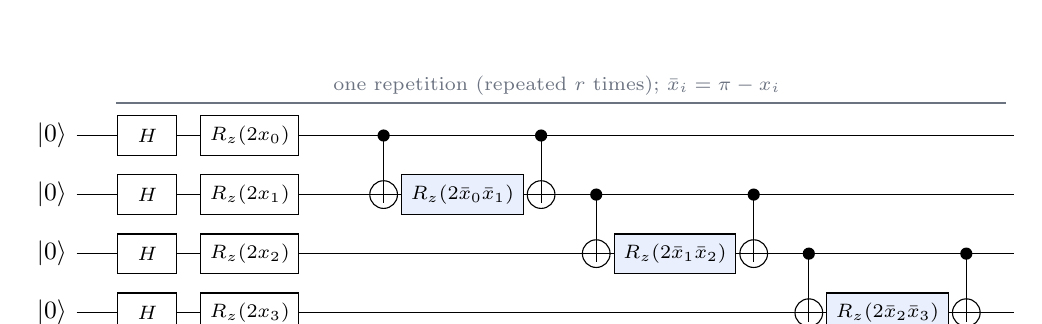
\begin{tikzpicture}[x=1cm,y=0.75cm,
  g/.style={draw,fill=white,minimum width=0.75cm,minimum height=0.5cm,font=\scriptsize},
  zz/.style={draw,fill=qblue!10,minimum width=1.25cm,font=\scriptsize}]
\foreach \q in {0,...,3}{
  \draw (-0.6,-\q) node[left]{\small$\ket{0}$} -- (11.3,-\q);
  \node[g] at (0.3,-\q) {$H$};
  \node[g] at (1.6,-\q) {$R_z(2x_\q)$};
}
\foreach \a/\xpos in {0/3.3,1/6.0,2/8.7}{
  \pgfmathtruncatemacro{\b}{\a+1}
  \fill (\xpos,-\a) circle (2.2pt);
  \draw (\xpos,-\a) -- (\xpos,-\b-0.15);
  \draw (\xpos,-\b) circle (5pt); \draw (\xpos-0.17,-\b)--(\xpos+0.17,-\b);
  \node[zz,minimum height=0.5cm] at (\xpos+1.0,-\b) {$R_z(2\bar x_\a\bar x_\b)$};
  \fill (\xpos+2.0,-\a) circle (2.2pt);
  \draw (\xpos+2.0,-\a) -- (\xpos+2.0,-\b-0.15);
  \draw (\xpos+2.0,-\b) circle (5pt); \draw (\xpos+1.83,-\b)--(\xpos+2.17,-\b);
}
\draw[decorate,thick,qgrey] (-0.1,0.55) -- (11.2,0.55);
\node[font=\scriptsize,qgrey] at (5.5,0.85) {one repetition (repeated $r$ times); $\bar x_i=\pi-x_i$};
\end{tikzpicture}
\caption{One repetition of the ZZ feature map with linear entanglement on 4 qubits. Every gate
except $H$ is diagonal in the computational basis.}
\label{fig:circuit}
\end{figure}

\subsection{Kernel concentration and bandwidth}
\label{sec:conc}
Quantum kernels have a characteristic failure mode called \emph{exponential concentration}~\cite{thanasilp2024}.
For expressive feature maps on many qubits, the states of two different inputs are nearly
orthogonal in the $2^n$-dimensional space, so $K(\bm a,\bm b)\approx 0$ for all $\bm a\ne\bm b$
and the Gram matrix approaches the identity. An SVM trained on $K\approx I$ can fit the training
set perfectly, but its decision function on new points is close to a constant. This is the
quantum analogue of an RBF kernel with $\gamma\to\infty$. On hardware it is worse, because
resolving values of order $2^{-n}$ needs exponentially many shots.

Shaydulin and Wild~\cite{shaydulin2022} and Canatar et al.~\cite{canatar2022} showed that
\emph{scaling the input}, $\bm x\mapsto\alpha\bm x$ with $\alpha<1$, acts as a bandwidth: it
moves the states closer together, restores off-diagonal mass, and can turn a kernel that does not
generalise into one that does. The original project had no such parameter. Every feature used the
full $[0,\pi]$ range ($\alpha=1$).

\subsection{When can a quantum kernel help?}
\label{sec:gd}
A quantum kernel can only beat classical methods if (a)~it cannot be computed efficiently
classically, \emph{and} (b)~it fits the data better than the classical kernels one would
actually use. Huang et al.~\cite{huang2021} made (b) testable with the \emph{geometric difference}
\begin{equation}
g(K_C\|K_Q)=\sqrt{\big\|\sqrt{K_Q}\,(K_C+\lambda I)^{-1}\sqrt{K_Q}\big\|_\infty},
\label{eq:gd}
\end{equation}
computed on the training Gram matrices, both normalised to trace $N$. If $g$ is small (close to 1),
then for \emph{every} labelling the classical kernel generalises about as well as the quantum one,
so no advantage is possible on this data. A potential advantage requires $g\gtrsim\sqrt N$. We
compute $g$ against the tuned RBF kernel for every run (Section~\ref{sec:evalsw}). Recent
large-scale benchmarking~\cite{bowles2024} also found that, under careful tuning, out-of-the-box
classical models usually match or beat quantum models on small tasks. That is one more reason to
give the classical baseline the same tuning budget as the quantum model.

\section{The Dataset in This Repository}
\label{sec:dataset}

\subsection{Where the data lives}
The repository holds no folder of raw CIC-DDoS2019 CSVs. All data is in one 33\,MB file,
\code{output.csv}, which \code{main.py} reads through \code{data\_loader.load\_csv()} (default path
\code{./output.csv}). It has 74{,}999 data lines and 88 columns: an index column
(\code{Unnamed: 0}), seven identifier columns (\code{Flow ID}, source/destination IP and port,
\code{Protocol}, \code{Timestamp}), 77 numeric CICFlowMeter features, \code{SimillarHTTP},
\code{Inbound} and \code{Label}.

\paragraph{Provenance.} Several clues show how the file was made. Four of its lines repeat the
header row (with \code{Label}=``Label''), so it is a concatenation of several CICFlowMeter CSVs.
The class names (\code{MSSQL}, \code{LDAP}, \code{Portmap}, \code{Syn}, \code{UDP}, without the
\code{DrDoS\_} prefix used in the January files) and the presence of \code{Portmap} match the
CSVs of the \emph{11 March} capture day, whose timestamps read \code{2018-11-03}. The paper
attributes these classes to the 12 January ``training day''; that should be corrected. Each attack
class contributes roughly 10--20k rows (Table~\ref{tab:dups}), and the \code{Unnamed: 0} index
values (up to 482{,}780) point back to positions in much larger source files. Most importantly,
each class covers a \emph{very short time window}: all 14{,}999 \code{Syn} flows fall within
1.1\,s, all \code{UDP} flows within 2\,s, and all \code{LDAP} flows within about 2 minutes. The
file is therefore a set of contiguous slices from each class's capture, not a random sample of
the full dataset.

\subsection{Class composition and duplicates}
After removing the four repeated header lines, 74{,}995 rows remain. The loader counts two rows
as duplicates when all 61 feature columns used by the paper and the label are equal. By that
definition, \textbf{49{,}393 rows (65.9\%) are exact duplicates} of an earlier row
(Table~\ref{tab:dups}).

\begin{table}[H]
\centering\small
\caption{Rows, duplicates and unique rows per class in \code{output.csv} (paper feature set).}
\label{tab:dups}
\begin{tabular}{lrrrr}
\toprule
Class & Rows & Duplicates & Unique & Duplicate share \\
\midrule
BENIGN & 5,126 & 786 & 4,340 & 15.3\% \\
LDAP & 9,931 & 9,353 & 578 & 94.2\% \\
MSSQL & 19,657 & 13,697 & 5,960 & 69.7\% \\
Portmap & 10,284 & 9,521 & 763 & 92.6\% \\
Syn & 14,999 & 8,706 & 6,293 & 58.0\% \\
UDP & 14,998 & 7,330 & 7,668 & 48.9\% \\
\midrule
Total & 74,995 & 49,393 & 25,602 & 65.9\% \\

\bottomrule
\end{tabular}
\end{table}

The reflection attacks are almost entirely repetitive: only 578 of 9{,}931 LDAP flows and 763 of
10{,}284 Portmap flows are distinct. This is expected, since an amplification attack replays
the same request millions of times and CICFlowMeter maps identical packet trains to identical
feature vectors. It has a direct consequence for evaluation. If duplicates are kept and the data
is split at random, a large share of test flows have an identical copy in the training set, and
the classifier only needs to look them up. Section~\ref{sec:impdata} measures this effect:
about 30\% of test rows.

The low number of unique LDAP and Portmap flows also caps the balanced multiclass sample size.
With deduplication, the smallest class (LDAP, 578 unique flows) limits a balanced 6-class sample
to at most $6\times578=3468$ rows.

\subsection{Features}
The original loader lists 61 numeric columns (the ``paper'' feature set). Twelve are constant
zero in this file: \code{Bwd PSH Flags}, \code{Fwd/Bwd URG Flags}, \code{FIN}, \code{PSH} and
\code{ECE Flag Count}, and all six \code{Bulk} statistics. That leaves \textbf{49 informative
features}, not the 58 stated in the paper. The original loader padded the matrix with zero
columns to reach exactly 58; those columns carry no information and are dropped by PCA anyway.
The ``all'' feature set adds 16 more columns (Subflow counts, \code{Init\_Win\_bytes\_forward/backward},
\code{act\_data\_pkt\_fwd}, \code{min\_seg\_size\_forward}, Active/Idle statistics). Identifier
columns (IPs, ports, timestamps, flow IDs) are never used: in this testbed they would reveal the
attack hosts and time windows and give a trivially perfect but meaningless classifier.

The rate columns \code{Flow Bytes/s} and \code{Flow Packets/s} contain $\pm\infty$ in about 2{,}650
rows (CICFlowMeter divides by a zero duration). Five rows are NaN. Both are set to 0.

\paragraph{Heavy tails.} Most features are extremely skewed. \code{Flow Bytes/s} ranges up to
$2.9\times10^{9}$. Under linear min--max scaling to $[0,\pi]$, 35\% of flows receive an angle
below 0.01\,rad (Figure~\ref{fig:skew}). Across all 49 informative features, the median of the
90th percentile after min--max scaling is only $0.0017$: for 69\% of the features, nine out of ten
flows end up in the bottom 5\% of the rotation range. Section~\ref{sec:impdata} explains why this
matters for angle encoding and how a signed log transform fixes it.

\begin{figure}[H]
\centering
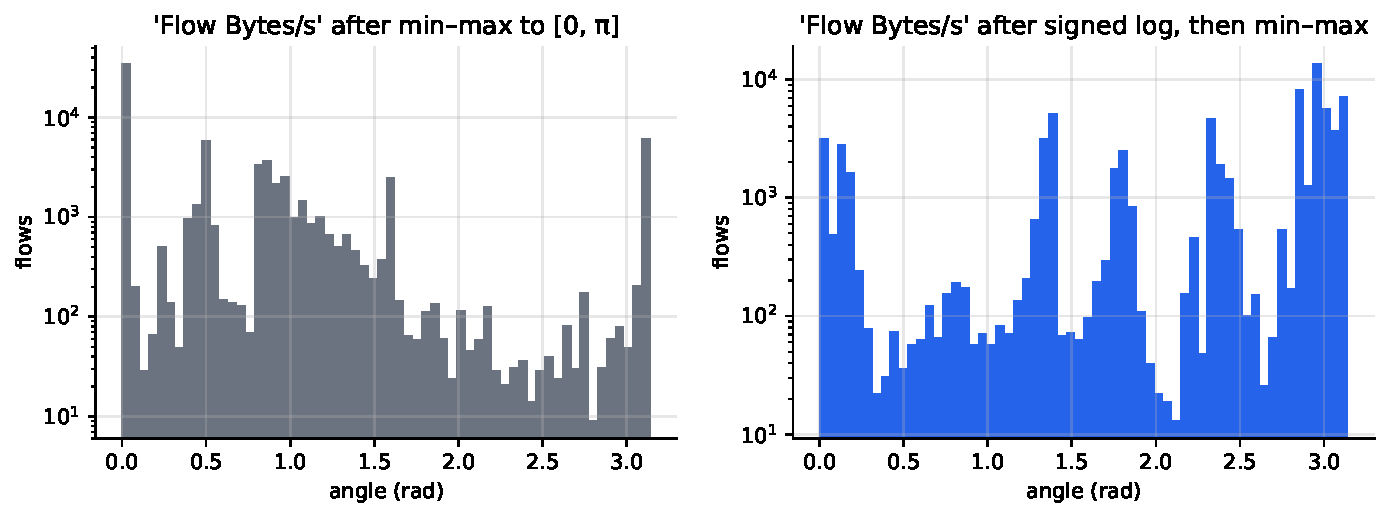
\includegraphics[width=\linewidth]{figures/skew.pdf}
\caption{Distribution of the rotation angle derived from \code{Flow Bytes/s} (log-scale
counts). Left: linear min--max, as in the original code; almost all mass sits at angle $\approx0$.
Right: after a signed $\log(1+|x|)$ transform the full $[0,\pi]$ range is used.}
\label{fig:skew}
\end{figure}

\subsection{Tasks}
\begin{itemize}
\item \textbf{Binary}: \code{BENIGN} (label 0) vs.\ any attack (label 1, ``DDoS''). Classes are
      balanced by undersampling. With deduplication the attack half is drawn from the pooled
      unique attack flows, which are dominated by UDP, Syn and MSSQL.
\item \textbf{Multiclass}: the six labels, BENIGN, LDAP, MSSQL, Portmap, Syn and UDP (alphabetical
      codes 0--5), undersampled to equal counts.
\end{itemize}
Both tasks use \code{--samples} (default 2000) as the total sample size, split 80/20 into
train/test with stratification. In multiclass mode that means 333 samples per class, 1{,}598
training samples and 400 test samples.

\section{The Original Pipeline and Its Audit}
\label{sec:original}

\subsection{Architecture}
The original code (preserved verbatim in \code{legacy/}) has three modules. Figure~\ref{fig:pipeline-old}
shows the data flow.

\begin{figure}[H]
\centering
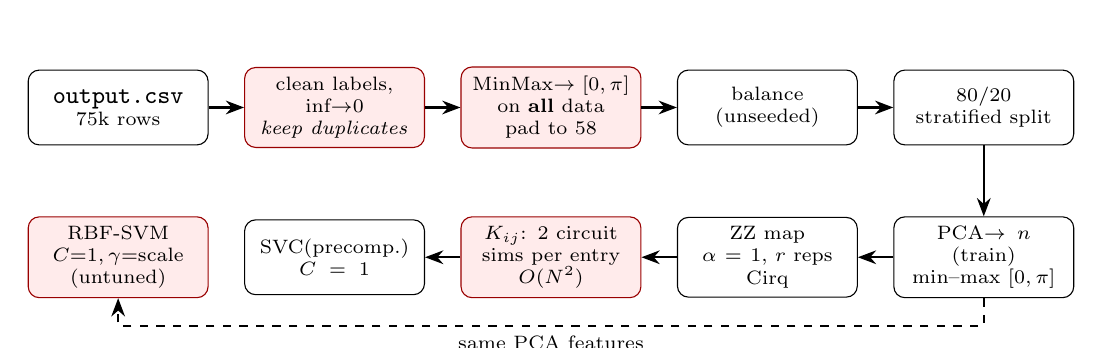
\begin{tikzpicture}[node distance=0.35cm and 0.45cm,
  box/.style={draw,rounded corners,fill=white,align=center,font=\scriptsize,minimum height=0.95cm,text width=2.05cm},
  bad/.style={box,fill=red!8,draw=red!60!black},
  arr/.style={-{Stealth},thick}]
\node[box] (csv) {\code{output.csv}\\75k rows};
\node[bad,right=of csv] (clean) {clean labels,\\inf$\to$0\\\textit{keep duplicates}};
\node[bad,right=of clean] (mm) {MinMax$\to[0,\pi]$\\on \textbf{all} data\\pad to 58};
\node[box,right=of mm] (bal) {balance\\(unseeded)};
\node[box,right=of bal] (split) {80/20\\stratified split};
\node[box,below=0.9cm of split] (pca) {PCA$\to n$\\(train)\\min--max $[0,\pi]$};
\node[box,left=of pca] (zz) {ZZ map\\$\alpha=1$, $r$ reps\\Cirq};
\node[bad,left=of zz] (ker) {$K_{ij}$: 2 circuit\\sims per entry\\$O(N^2)$};
\node[box,left=of ker] (svc) {SVC(precomp.)\\$C=1$};
\node[bad,left=of svc] (rbf) {RBF-SVM\\$C{=}1,\gamma$=scale\\(untuned)};
\draw[arr] (csv)--(clean); \draw[arr] (clean)--(mm); \draw[arr] (mm)--(bal); \draw[arr] (bal)--(split);
\draw[arr] (split)--(pca); \draw[arr] (pca)--(zz); \draw[arr] (zz)--(ker); \draw[arr] (ker)--(svc);
\draw[arr,dashed] (pca.south) -- ++(0,-0.35) -| node[pos=0.25,below,font=\scriptsize]{same PCA features} (rbf.south);
\end{tikzpicture}
\caption{Original pipeline. Red boxes mark steps changed by this work.}
\label{fig:pipeline-old}
\end{figure}

\paragraph{\code{data\_loader.py}.} \code{load\_csv()} reads the CSV, strips column names, removes
repeated header rows, and draws up to $3\times$\code{max\_samples} rows at random
(\code{random\_state=42}). It builds binary or multiclass labels, selects up to 61 named feature
columns, replaces $\pm\infty$/NaN by 0, drops zero-variance columns, and pads or trims to exactly 58
columns. It then undersamples each class to $\min(\text{smallest class},\,\text{max\_samples}/k)$
using the \emph{unseeded} global \code{np.random}. Finally it fits a \code{MinMaxScaler} to $[0,\pi]$
on \emph{all} remaining rows and returns them.

\paragraph{\code{qsvm.py}.} \code{ZZFeatureMap.build\_encoding\_circuit()} builds the circuit of
Figure~\ref{fig:circuit} in Cirq. \code{build\_kernel\_circuit()} builds $U^\dagger(\bm a)U(\bm b)$
plus measurement, for the sampling mode. \code{QuantumKernel.\_kernel\_statevector(a,b)} simulates
\emph{both} circuits with \code{cirq.Simulator} and returns $|\langle\psi_a|\psi_b\rangle|^2$.
\code{compute\_kernel\_matrix()} loops over all $(i,j)$ pairs, using symmetry for the training
matrix. \code{QSVM.fit()} fits PCA to \code{n\_qubits} components on the training rows, rescales
each component to $[0,\pi]$ with training min/max, computes $K_{\text{train}}$ and fits
\code{SVC(kernel='precomputed', C=1, probability=True)}. \code{predict()} and
\code{predict\_proba()} \emph{each} rebuild the full test kernel.

\paragraph{\code{main.py}.} \code{run\_pipeline()} loads the data, splits it 80/20 (stratified,
\code{random\_state=42}), truncates the training set to 3000 rows, trains the QSVM, then trains
\code{SVC(kernel='rbf', C=1, gamma='scale')} on standardised PCA features (same projection) and
prints accuracy, a classification report, timings and a 4-panel figure (two confusion matrices,
ROC, accuracy bars).

\subsection{Reported results}
Table~\ref{tab:paper} reproduces the paper's headline numbers. Only the ZZ method exists in the
code. The Analytical and Sampling variants were run from earlier versions that are not in the
repository.

\begin{table}[H]
\centering\small
\caption{Results reported in the paper~\cite{ourpaper} (single run each).}
\label{tab:paper}
\begin{tabular}{llccc c}
\toprule
Method & Mode & QSVM acc. & SVM acc. & QSVM AUC & $N_\text{test}$ \\
\midrule
Analytical ($R_x$, 16q) & binary & 97.57\% & 98.54\% & 0.987 & 1028 \\
Analytical ($R_x$, 16q) & multiclass & 89.63\% & 87.68\% & -- & 3084 \\
Sampling (1024 shots)   & binary & 98.54\% & 98.54\% & 0.992 & 1028 \\
Sampling (1024 shots)   & multiclass & 89.63\% & 87.68\% & -- & 3084 \\
ZZ (8q, 2 reps)         & binary & \textbf{98.79\%} & 96.97\% & 0.999 & 822 \\
ZZ (16q, 1 rep)         & multiclass & \textbf{92.00\%} & 80.00\% & -- & 996 \\
\bottomrule
\end{tabular}
\end{table}

\subsection{Audit findings}
We read every line of the three modules and checked the data file. Table~\ref{tab:audit} lists
the issues found, ordered roughly by how much they can change the conclusions.

\begin{table}[H]
\centering\small
\caption{Issues found in the original pipeline.}
\label{tab:audit}
\begin{tabularx}{\linewidth}{c l X c}
\toprule
\# & Issue & Effect & Severity \\
\midrule
I1 & Exact duplicates kept & 65.9\% of rows are duplicates; $\approx$30\% of test flows have a
  training twin (measured). Accuracy is inflated by memorisation. & High \\
I2 & Untuned, unequal baselines & QSVM and RBF both fixed at $C=1$; RBF $\gamma$ fixed at
  \code{'scale'}. The comparison measures default settings, not models. & High \\
I3 & Kernel concentration & 16-qubit ZZ kernel with $\alpha=1$: median off-diagonal entry
  $\approx 2\times10^{-5}$, 84--89\% of entries below $10^{-3}$, so $K\approx I$ (measured in Section~\ref{sec:results}). No bandwidth control. & High \\
I4 & Cost $2N^2$ simulations & Two full circuit simulations per kernel entry, and the test kernel
  is computed twice. A 1600-sample, 16-qubit run is estimated at $\approx$44\,h. & High (practical) \\
I5 & Global MinMax before split & Test-set min/max leak into the training features. & Medium \\
I6 & Linear encoding of heavy tails & For most features, 90\% of flows occupy $<5\%$ of
  $[0,\pi]$, so qubits receive near-constant angles. & Medium \\
I7 & Single run, no significance & Differences of 1--2 points on 400--1000 test flows are within
  sampling noise. There are no error bars and no tests. & Medium \\
I8 & Non-reproducible sampling & Class balancing uses unseeded \code{np.random}; Platt scaling
  is unseeded. Each run draws different data. & Medium \\
I9 & Inconsistent sample sizes & The paper compares methods on different $N$ (822 vs.\ 1028 test). & Medium \\
I10 & Missing methods & The Analytical and Sampling kernels in the paper are not in the code. & Medium \\
I11 & Narrow metrics & Accuracy only. IDS operators care about false-alarm rate and detection
  rate. Multiclass AUC is not reported. & Low \\
I12 & Cosmetic & Zero-padding to 58 columns; hard-coded ``58 $\to$'' message; silent truncation
  to 3000 training rows. & Low \\
I13 & Pre-sampling shrinks the data & $3\times$\code{max\_samples} random rows are drawn \emph{before}
  balancing. BENIGN is only 6.8\% of the file, so \code{--samples 2000} yields 411 BENIGN rows and
  822 binary samples in total (165 test flows). & Medium \\
\bottomrule
\end{tabularx}
\end{table}

\paragraph{How small the binary test set was.} Running the original loader confirms I13: with the
default \code{--samples 2000} it returns exactly 822 binary samples, the $N$ quoted in the paper for
the ZZ binary experiment, so the test split had 165 flows. The reported 98.79\% vs.\ 96.97\% is then
$163/165$ vs.\ $160/165$, a difference of \textbf{three test flows}. Even if all three were cases
where only the QSVM was right, the exact McNemar test would give $p=0.25$. The multiclass figures
(92.00\% vs.\ 80.00\%, $N=996=6\times166$) correspond to a 200-flow test set. The 12-point gap is
large, but it comes from a single split with the issues above.

None of these issues is unusual. Duplicate leakage in particular is a well-documented trap in
intrusion-detection benchmarks~\cite{engelen2021,kaufman2012}, and untuned baselines are the most
common cause of overstated quantum advantage~\cite{bowles2024}. The core idea and the quantum
code itself are sound. The fast engine reproduces the original kernel values exactly
(Section~\ref{sec:verify}).

\section{Improvements I: Data Integrity}
\label{sec:impdata}

Figure~\ref{fig:pipeline-new} shows the improved pipeline. Table~\ref{tab:changes} maps every
audit finding to its fix and the file that implements it. The next four sections describe the
changes in detail.

\begin{figure}[H]
\centering
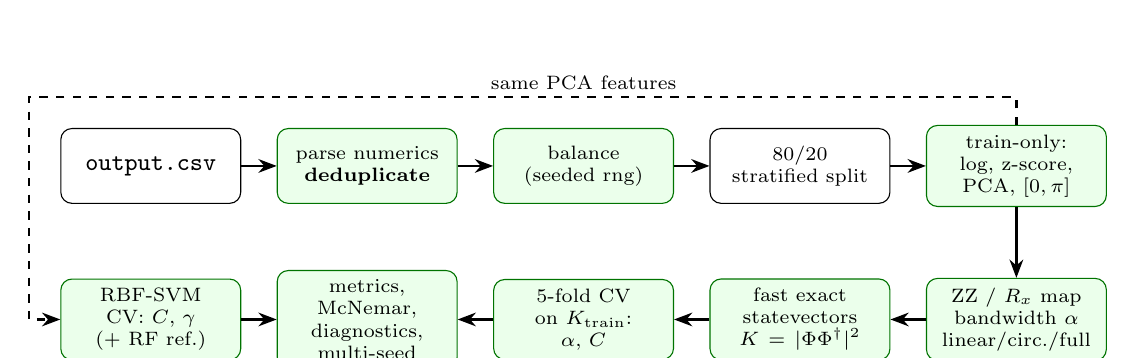
\begin{tikzpicture}[node distance=0.35cm and 0.45cm,
  box/.style={draw,rounded corners,fill=white,align=center,font=\scriptsize,minimum height=0.95cm,text width=2.05cm},
  new/.style={box,fill=green!8,draw=green!45!black},
  arr/.style={-{Stealth},thick}]
\node[box] (csv) {\code{output.csv}};
\node[new,right=of csv] (clean) {parse numerics\\\textbf{deduplicate}};
\node[new,right=of clean] (bal) {balance\\(seeded rng)};
\node[box,right=of bal] (split) {80/20\\stratified split};
\node[new,right=of split] (prep) {train-only:\\log, z-score,\\PCA, $[0,\pi]$};
\node[new,below=0.9cm of prep] (zz) {ZZ / $R_x$ map\\bandwidth $\alpha$\\linear/circ./full};
\node[new,left=of zz] (ker) {fast exact\\statevectors\\$K=|\Phi\Phi^\dagger|^2$};
\node[new,left=of ker] (cv) {5-fold CV\\on $K_\text{train}$:\\$\alpha$, $C$};
\node[new,left=of cv] (eval) {metrics, McNemar,\\diagnostics,\\multi-seed};
\node[new,left=of eval] (rbf) {RBF-SVM\\CV: $C$, $\gamma$\\(+ RF ref.)};
\coordinate (L) at ([xshift=-4mm]csv.west);
\draw[arr] (csv)--(clean); \draw[arr] (clean)--(bal); \draw[arr] (bal)--(split); \draw[arr] (split)--(prep);
\draw[arr] (prep)--(zz); \draw[arr] (zz)--(ker); \draw[arr] (ker)--(cv); \draw[arr] (cv)--(eval);
\draw[arr] (rbf)--(eval);
\draw[arr,dashed] (prep.north) -- ++(0,0.35) node[above left,font=\scriptsize,pos=1]{} -| (L) |- (rbf.west);
\node[font=\scriptsize,above] at ($(prep.north)!0.5!(csv.north)+(0,0.35)$) {same PCA features};
\end{tikzpicture}
\caption{Improved pipeline. Green boxes are new or changed. Every fitted statistic comes from the
training split only.}
\label{fig:pipeline-new}
\end{figure}

\begin{table}[H]
\centering\small
\caption{Audit finding $\to$ change $\to$ location.}
\label{tab:changes}
\begin{tabularx}{\linewidth}{c X l}
\toprule
\# & Change & Where \\
\midrule
I1 & Drop exact duplicate (features, label) rows before sampling; report the train/test overlap & \code{data\_loader.py} \\
I2 & 5-fold CV grid search on the training set for QSVM ($\alpha$, $C$) and RBF ($C$, $\gamma$), same metric and folds & \code{evaluation.py} \\
I3 & Bandwidth $\alpha$ (input scaling) in all feature maps; concentration diagnostics & \code{qsvm.py}, \code{evaluation.py} \\
I4 & One simulation per sample plus a Gram product; fast exact NumPy engine; state cache & \code{qsvm.py} \\
I5 & All scaling/PCA fitted on training rows only; test values clipped to $[0,\pi]$ & \code{preprocessing.py} \\
I6 & Signed $\log(1+|x|)$ before standardisation and PCA & \code{preprocessing.py} \\
I7 & \code{--seeds}: repeat over seeds, report mean $\pm$ std; exact McNemar test per seed & \code{main.py}, \code{evaluation.py} \\
I8 & Seeded \code{default\_rng}; seeded Platt scaling, PCA and CV & all modules \\
I9 & All methods share one loader, one split and one preprocessing per seed & \code{main.py}, \code{benchmark.py} \\
I10 & \code{--kernel rx} (closed form) and \code{--sampling} (shots) added to the pipeline & \code{qsvm.py} \\
I11 & Balanced accuracy, macro-F1, MCC, AUC (binary and OvR), false-alarm and detection rates & \code{evaluation.py} \\
I12 & No padding; real feature counts reported; no silent truncation & \code{data\_loader.py}, \code{main.py} \\
I13 & Balance from the full (deduplicated) pool, so \code{--samples} is the real sample size & \code{data\_loader.py} \\
\bottomrule
\end{tabularx}
\end{table}

\subsection{Duplicate removal (I1)}
\paragraph{Problem.} With duplicates kept, many test flows are byte-identical to training flows.
\code{data\_loader.duplicate\_overlap()} measures this directly by hashing every training row and
counting test rows found in the set. For the original protocol it reports
\textbf{28--30\%} of test rows in the binary task (Table~\ref{tab:ablation}). A kernel
classifier gets those rows right automatically: $K(\bm x,\bm x)=1$ is the largest possible kernel
value, so the training twin dominates the decision function.

\paragraph{Change.} \code{load\_csv(dedup=True)} (the default) removes rows whose 61 feature values
\emph{and} task label equal those of an earlier row, before any sampling:
\begin{verbatim}
    key = X_df.copy(); key["__label"] = y_all
    keep = ~key.duplicated().values
\end{verbatim}
The key uses the label of the task (\code{y\_all}), not the raw attack name: in binary mode an
LDAP flow and an identical Portmap flow are both ``DDoS'', so the second one is a duplicate
(175 extra rows). Identical feature vectors with \emph{different} task labels (177 rows in
multiclass mode, 2 in binary mode) are kept. They are genuine
ambiguity, not leakage. \code{--keep-duplicates} restores the old behaviour for comparison.
After deduplication the overlap falls to 0--0.25\% (a handful of rows that differ only in
dropped zero-variance columns).

\paragraph{Why it matters for the conclusions.} Duplicates do not affect all models equally. A
kernel that is very sharp ($K\approx I$ off the diagonal, as with the untuned 16-qubit ZZ map)
behaves almost like a nearest-neighbour lookup. It benefits \emph{most} from exact twins and is
hurt most on genuinely new flows. Leakage can therefore create a spurious advantage for exactly
the most ``quantum'' kernel.

\subsection{Leakage-free preprocessing (I5)}
\paragraph{Problem.} The original loader called \code{MinMaxScaler().fit\_transform(X)} on all
sampled rows, then \code{main.py} split them. Each feature's minimum and maximum therefore
included test rows. With heavy-tailed features the maximum is often a single extreme flow, so
whether that flow lands in train or test changes the scale of every training feature.

\paragraph{Change.} \code{data\_loader.py} now returns raw, unscaled features. A new class,
\code{QuantumPreprocessor} in \code{preprocessing.py}, is fitted on the training split only, inside
\code{QSVM.fit()}. Its \code{transform()} applies the stored statistics to the test set and clips
out-of-range angles to $[0,\pi]$. The classical baselines use \code{transform\_pca()} of the
\emph{same} fitted object, so both models see identical information. The original behaviour is
kept as \code{LegacyPreprocessor} plus \code{legacy\_global\_scale()}, selected with
\code{--legacy-scaling}.

\subsection{Signed log transform (I6)}
\paragraph{Problem.} Angle encoding maps each feature to a rotation. If 90\% of flows fall within
0.002\,rad of each other, the corresponding qubit is in essentially the same state for all of
them, and the kernel cannot tell them apart along that direction. PCA does not help, because it
is dominated by the few extreme flows that define the variance.

\paragraph{Change.} Before standardisation and PCA, every feature is transformed by
\begin{equation}
x\mapsto \operatorname{sign}(x)\,\log(1+|x|).
\end{equation}
This is monotone, defined for zero and negative values (\code{Fwd Header Length} is negative in
12{,}592 rows, an artefact of CICFlowMeter), and compresses nine orders of magnitude into about 22 units.
Figure~\ref{fig:skew} shows the result for \code{Flow Bytes/s}: the median angle moves from
0.45 to 2.86\,rad and the fraction of flows below 0.01\,rad drops from 35\% to 4\%. The pipeline
is then: drop zero-variance columns $\to$ signed log $\to$ \code{StandardScaler} $\to$
\code{PCA}($n$) $\to$ per-component min--max to $[0,\pi]$, all fitted on training data.
\code{--no-log} disables the transform for ablation.

\subsection{Reproducible sampling and real sample sizes (I8, I12, I13)}
All randomness now flows from the \code{--seeds} values: \code{np.random.default\_rng(seed)} for
balancing, \code{random\_state=seed} for the split, PCA, \code{StratifiedKFold}, Platt scaling, the
Random Forest and the shot-noise generator. Two runs with the same seed produce byte-identical
results; this is verified in \code{tests/test\_core.py::test\_dedup\_and\_reproducible}. Classes are
balanced by drawing from the whole (deduplicated) pool of each class, so \code{--samples 2000} now
really gives 2000 samples (1000 per class in binary mode, 333 per class in multiclass mode)
instead of 822. \code{--legacy} uses the same sampler, so that the original and improved protocols
are always compared on the same number of flows. Numeric
parsing uses \code{pd.to\_numeric(errors='coerce')} so stray strings cannot crash the cast. Zero
padding to 58 columns was removed, and the true number of features entering PCA is printed.

\section{Improvements II: Computation}
\label{sec:impcompute}

The original kernel code is correct but very slow. It is so slow that it ruled out the
experiments needed to answer the project's own research question: repeated runs, tuning,
ablations, and realistic training-set sizes at 16 qubits. This section describes three changes
that keep the exact same kernel values while removing the bottleneck.

\subsection{Simulate each sample once (statevector caching)}
\paragraph{Problem.} \code{\_kernel\_statevector(a, b)} simulated $U(\bm a)\ket0$ and
$U(\bm b)\ket0$ from scratch for every pair. For $N$ training and $M$ test samples the original
code performed
\begin{equation}
\underbrace{2\cdot\tfrac{N(N+1)}{2}}_{K_\text{train}}+\underbrace{2\cdot 2MN}_{K_\text{test}\ \text{in predict and predict\_proba}}
\end{equation}
circuit simulations: about 5.1 million for $N=1600$, $M=400$. Yet $\ket{\phi(\bm x)}$ depends
only on $\bm x$.

\paragraph{Change.} \code{QuantumKernel.states(X)} returns the matrix $\Phi_X\in\mathbb{C}^{N\times2^n}$
whose rows are the feature states. The whole kernel matrix is then one matrix product:
\begin{equation}
K(X,Y)=\big|\,\overline{\Phi_X}\,\Phi_Y^{\top}\big|^{\circ2}\qquad(\text{element-wise squared modulus}).
\label{eq:gram}
\end{equation}
This needs $N+M$ state preparations and one complex GEMM (\code{cgemm} in OpenBLAS, multithreaded),
computed in row blocks of 512 to bound memory. The most recent two state matrices are memoised.
When the test kernel is built, the training states are reused rather than re-simulated, and
\code{QSVM.predict}, \code{predict\_proba} and \code{decision\_function} share one cached test
kernel. With the Cirq backend this alone cuts the 16-qubit cost from about 44 hours to about
a minute (Table~\ref{tab:speed}).

\subsection{An exact fast engine for the ZZ feature map}
Cirq is a general-purpose simulator. It applies each of the $\approx\!4n$ gates per repetition as
a separate tensor contraction, with Python overhead per gate and per circuit. The ZZ map has
special structure that a dedicated engine can use.

\begin{proposition}
Let $s_i(z)=1-2z_i$ and
\begin{equation}
\Phi_{\bm x}(z)=\sum_{i=1}^n x_i\,s_i(z)+\sum_{(i,j)\in E}(\pi-x_i)(\pi-x_j)\,s_i(z)s_j(z).
\label{eq:phase}
\end{equation}
Then one repetition of the ZZ map is $U=D_{\bm x}H^{\otimes n}$ with $D_{\bm x}\ket z=e^{-i\Phi_{\bm x}(z)}\ket z$,
and the feature state after $r$ repetitions is
\begin{equation}
\ket{\phi_r(\bm x)}=D_{\bm x}H^{\otimes n}\cdots D_{\bm x}H^{\otimes n}\ket{0^n},\qquad
\ket{\phi_1(\bm x)}=2^{-n/2}\sum_z e^{-i\Phi_{\bm x}(z)}\ket z .
\end{equation}
\end{proposition}
\begin{proof}
$R_z(2x_i)$ acts on $\ket z$ as $e^{-ix_is_i(z)}$. By Eq.~\eqref{eq:zzgate}, the gate block for
pair $(i,j)$ acts as $e^{-i(\pi-x_i)(\pi-x_j)s_i(z)s_j(z)}$. All these operators are diagonal, so
they commute and their phases add, giving $D_{\bm x}$. Finally,
$H^{\otimes n}\ket{0^n}=2^{-n/2}\sum_z\ket z$.
\end{proof}

\paragraph{Implementation} (\code{FastZZStatevector} in \code{qsvm.py}).
\begin{enumerate}
\item \textbf{Phase table.} Precompute the sign matrix $S\in\{\pm1\}^{2^n\times n}$, with qubit 0
      as the most significant bit to match Cirq's ordering, and the pair-product matrix
      $S_P\in\{\pm1\}^{2^n\times|E|}$. For a batch of inputs $X$ (rows $\bm x$), all phases are
      two real matrix products:
      $\Phi = X S^\top + W S_P^\top$, where $W_{b,(i,j)}=(\pi-x_{b,i})(\pi-x_{b,j})$.
\item \textbf{First repetition} is free: $\psi=2^{-n/2}e^{-i\Phi}$, element-wise.
\item \textbf{Hadamard layers.} $H^{\otimes n}=H^{\otimes n_1}\otimes H^{\otimes n_2}$ with
      $n_1=\lfloor n/2\rfloor$. Reshaping $\psi$ into a $2^{n_1}\times2^{n_2}$ matrix $M$ (row-major)
      gives $(A\otimes B)\,\mathrm{vec}(M)=\mathrm{vec}(AMB^\top)$. Each layer is therefore two
      small batched matrix multiplications with $256\times256$ matrices at $n=16$, instead of a
      $65536\times65536$ operator or 16 strided butterfly passes.
\item Multiply by $D_{\bm x}$ again and repeat.
\end{enumerate}
The cost per sample is $O(2^n(n+|E|))$ for the phases and $O(2^n(2^{n_1}+2^{n_2}))$ per Hadamard
layer. Everything is vectorised over batches of 128 samples. States are stored as
\code{complex64}, the same precision Cirq uses by default.

\begin{algorithm}[H]
\caption{Training kernel with the fast engine}
\begin{algorithmic}
\STATE \textbf{input:} angles $A\in[0,\pi]^{N\times n}$, bandwidth $\alpha$, reps $r$, pairs $E$
\STATE $X\leftarrow\alpha A$
\FOR{each batch $B$ of 128 rows of $X$}
  \STATE $\Phi\leftarrow XS^\top+W(X)S_P^\top$;\quad $D\leftarrow e^{-i\Phi}$
  \STATE $\psi\leftarrow 2^{-n/2}D$
  \FOR{$k=2$ \TO $r$}
     \STATE $\psi\leftarrow \mathrm{vec}\big(H^{\otimes n_1}\,\mathrm{mat}(\psi)\,(H^{\otimes n_2})^{\top}\big)\odot D$
  \ENDFOR
  \STATE store $\psi$ as rows of $\Phi_X$
\ENDFOR
\STATE $K\leftarrow|\overline{\Phi_X}\Phi_X^\top|^{\circ 2}$;\quad symmetrise;\quad set $\operatorname{diag}(K)=1$
\end{algorithmic}
\end{algorithm}

\subsection{Other kernels on the same engine}
\paragraph{Separable $R_x$ kernel.} With the fast backend, Eq.~\eqref{eq:rxkernel} is evaluated
in closed form with broadcasting, in row blocks of 256. With the Cirq backend the product state
is simulated, which serves as a cross-check.

\paragraph{Finite shots.} Running $U^\dagger(\bm a)U(\bm b)$ for $s$ shots and counting the
all-zero outcomes gives a count distributed exactly as $\text{Binomial}(s, K(\bm a,\bm b))$: each
shot is an independent Bernoulli trial with success probability $|\bra{0^n}U^\dagger(\bm a)U(\bm b)\ket{0^n}|^2=K(\bm a,\bm b)$.
The fast backend therefore computes the exact kernel and draws
\begin{equation}
\hat K_{ij}=\frac1s\,\text{Binomial}\big(s,K_{ij}\big),
\end{equation}
independently for each upper-triangular entry, then mirrors it. This has \emph{the same
distribution} as the original sampling method at a tiny fraction of the cost. The real circuit
path is still available with \code{--backend cirq --sampling}. The estimator is unbiased
(verified in \code{test\_shot\_noise\_is\_unbiased}). The resulting matrix need not be PSD;
libsvm tolerates mildly indefinite kernels.

\subsection{Verification}
\label{sec:verify}
Speed is only useful if the numbers are unchanged. \code{tests/test\_core.py} checks:
\begin{itemize}
\item fast statevectors equal Cirq's (\code{atol} $10^{-5}$) for linear, circular and full
      entanglement, 2 and 3 repetitions, $\alpha=1$ and $\alpha=0.3$, and for the $R_x$ map.
      Observed maximum deviation: $2.4\times10^{-7}$, i.e.\ \code{float32} rounding;
\item the new kernel value equals the value from the \emph{original, unmodified}
      \code{legacy/qsvm.py} (\code{QuantumKernel(6,2).compute\_kernel\_value}) to 5 decimals;
\item Gram matrices are symmetric with unit diagonal, and their smallest eigenvalue is
      $>-10^{-5}$ (PSD up to rounding).
\end{itemize}
\code{main.py --backend cirq} and \code{--backend fast} produce identical predictions
(TESTING.md \S6).

\subsection{Speed}
Table~\ref{tab:speed} and Figure~\ref{fig:speed} compare the cost of the training ($1600^2$) plus
test ($400\times1600$) kernels. ``Original'' is extrapolated from the measured per-entry time of
\code{legacy/qsvm.py} times the number of entries it evaluates. ``Cirq cached'' is the measured
per-state Cirq time times 2000 states, plus the measured Gram-product time. ``Fast'' is measured
end to end.

\begin{table}[H]
\centering\small
\caption{Kernel computation cost, $N_\text{train}=1600$, $N_\text{test}=400$, 2 repetitions, linear
entanglement (8-core CPU). Legacy sampling uses 1024 shots per entry.}
\label{tab:speed}
\begin{tabular}{rrrrrrr}
\toprule
Qubits & Original/entry & Original total & Orig.\ sampling & Cirq cached & Fast & Speed-up \\
\midrule
4 & 8.6 ms & 6.1 h & 8.1 h & 8.5 s & 0.06 s & 344,270$\times$ \\
8 & 24.7 ms & 17.6 h & 16.9 h & 17.3 s & 0.16 s & 392,457$\times$ \\
12 & 34.3 ms & 24.4 h & -- & 27.7 s & 0.88 s & 99,298$\times$ \\
16 & 61.6 ms & 43.8 h & -- & 67.5 s & 26.41 s & 5,969$\times$ \\

\bottomrule
\end{tabular}
\end{table}

\begin{figure}[H]
\centering
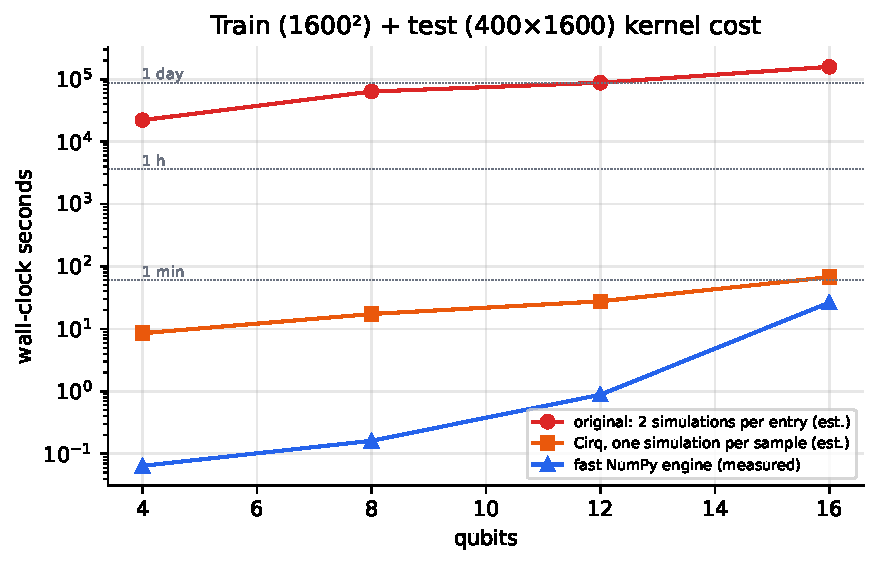
\includegraphics[width=0.72\linewidth]{figures/speed.pdf}
\caption{Wall-clock cost of a full train+test kernel (log scale). Original and Cirq-cached values
are estimates from measured unit costs; fast-engine values are measured end to end.}
\label{fig:speed}
\end{figure}

At 16 qubits the fast engine is limited by memory bandwidth: 2000 states $\times$ 65{,}536
amplitudes $\times$ 8 bytes is about 1\,GB, and the Gram product is about $1.7\times10^{11}$
complex multiply-adds. It is still roughly 6{,}000 times faster than the original, which is what
makes the 5-seed, cross-validated experiments in Section~\ref{sec:results} feasible.

\section{Improvements III: Modelling}
\label{sec:impmodel}

\subsection{Kernel bandwidth $\alpha$ (I3)}
\paragraph{Problem.} With $n$ qubits and inputs spread over $[0,\pi]$, the ZZ feature states of two
different flows are nearly orthogonal. Roughly, each qubit and each pair contributes an
independent ``random'' phase, and the overlap of two random states in dimension $2^n$ is of order
$2^{-n}$. The experiments confirm this: at 16 qubits with $\alpha=1$ and 2 repetitions, the
\emph{median} off-diagonal training kernel entry is about $2\times10^{-5}$ and 84--89\% of entries
are below $10^{-3}$. The mean is higher (about 0.03, Table~\ref{tab:bandwidth}) only because a
few near-identical flows still overlap strongly. An SVM can still
\emph{separate} the training set with such a kernel, but each test prediction is then decided by
a handful of nearest training points, and the kernel's geometry carries little information.

\paragraph{Change.} All feature maps now take a bandwidth parameter. Angles from preprocessing
are multiplied by $\alpha$ before encoding:
\begin{equation}
\ket{\phi_\alpha(\bm\theta)}=U(\alpha\bm\theta)\ket{0^n},\qquad \bm\theta\in[0,\pi]^n .
\end{equation}
Small $\alpha$ moves all states towards $U(\bm 0)\ket{0^n}$, raising off-diagonal kernel values.
In the limit $\alpha\to0$ the kernel tends to the constant 1. For the separable $R_x$ map,
$\alpha$ is exactly an RBF-like length-scale: $\cos^2(\alpha\Delta/2)\approx e^{-\alpha^2\Delta^2/4}$
for small $\alpha\Delta$. For the ZZ map, the pair term
$(\pi-\alpha\theta_i)(\pi-\alpha\theta_j)=\pi^2-\alpha\pi(\theta_i+\theta_j)+\alpha^2\theta_i\theta_j$
shows that $\alpha$ also controls how strongly the \emph{product} (entangling) terms depend on the
data, relative to the linear ones. $\alpha=1$ reproduces the original circuit exactly
(\code{ZZFeatureMap} and the fast engine both take \code{alpha}).

\subsection{Cross-validated tuning with equal budgets (I2)}
\paragraph{Problem.} With $C=1$ and a fixed scale for both models, the comparison measures how
well two \emph{default settings} happen to suit this dataset. RBF-SVM accuracy is very sensitive to
$\gamma$ and $C$. The default \code{gamma='scale'} ($1/(d\cdot\mathrm{Var}(X))$) is a heuristic, not
an optimum.

\paragraph{Change.} \code{evaluation.tune\_quantum()} performs a grid search over
$\alpha\in\{0.05,0.1,0.2,0.4,1.0\}$ and $C\in\{0.1,1,10,100\}$, scoring \emph{macro-F1} by 5-fold
stratified CV \emph{on the training split only}. The expensive part, the kernel, is computed once
per $\alpha$. Every $C$ and every fold then reuses sub-blocks $K[\text{tr},\text{tr}]$ and
$K[\text{va},\text{tr}]$ of that one matrix, so the search costs 5 kernel computations rather than
100 fits' worth. \code{tune\_rbf()} runs \code{GridSearchCV} for the RBF-SVM over the same
$C$ grid and $\gamma\in\{\text{scale},0.01,0.03,0.1,0.3,1\}$, with the same folds, metric and seed.
The best configuration is refitted on the full training split and evaluated once on the test set.
Both models get 20--24 candidate configurations: an equal budget.

\begin{verbatim}
alpha, C, K_train, table = tune_quantum(
    lambda a: make_kernel(a).compute_kernel_matrix(A_train, verbose=False),
    y_train, args.alphas, args.Cs, seed=seed)
\end{verbatim}

\code{--no-tune --alpha A --C C} fixes the values instead. \code{--alphas} and \code{--Cs} change
the grids.

\subsection{Entanglement topology and depth}
\code{entangling\_pairs(n, entanglement)} generalises the hard-coded adjacent pairs:
\code{linear} $\{(i,i{+}1)\}$ (original, $n-1$ pairs), \code{circular} (adds $(n{-}1,0)$), and
\code{full} (all $\binom n2$ pairs, the default in Qiskit's \code{ZZFeatureMap}). Both the Cirq
circuit builder and the fast engine use the same pair list, and \code{--n-reps} sets the depth. These
options answer the paper's ``higher-order entanglement'' future-work item within the existing
circuit family.

\subsection{All three paper methods in one pipeline (I10)}
\code{--kernel rx} selects the separable $R_x$ map (Method 1), and \code{--sampling --shots s} adds
finite-shot estimation to any kernel (Method 2). Together with the default ZZ map (Method 3), all
methods now share one loader, one split per seed, one preprocessing object and one tuning
protocol. The paper's comparisons used different $N$ for different methods (822 vs.\ 1028 binary
test samples); here every method sees exactly the same flows.

\subsection{Stronger classical references}
Besides the tuned RBF-SVM on the \emph{same} PCA features, which isolates the effect of the kernel,
\code{--extra-baselines} trains a Random Forest~\cite{breiman2001} (300 trees) on \emph{all}
raw features without PCA. This is a typical practical NIDS baseline. It answers a different
question: how much accuracy is left on the table by compressing to $n$ components at all?

\section{Improvements IV: Evaluation and Software}
\label{sec:evalsw}

\subsection{Metrics (I11)}
\code{evaluation.classification\_metrics()} reports, for every model and seed:
\begin{itemize}
\item \textbf{Accuracy} and \textbf{balanced accuracy} (mean per-class recall).
\item \textbf{Macro-F1}: the unweighted mean of per-class F1. It is the CV selection criterion,
      because it penalises neglecting any class.
\item \textbf{MCC} (Matthews correlation): a single-number summary that stays informative under
      imbalance.
\item \textbf{ROC-AUC}. In binary mode it is computed from \code{decision\_function}, the raw SVM
      margin, rather than from Platt probabilities, so it reflects the model and not the
      calibration fold. In multiclass mode it is the macro one-vs-rest AUC from \code{predict\_proba}.
      The paper reported no multiclass AUC.
\item \textbf{False-alarm rate} (FAR): the fraction of BENIGN flows flagged as any attack.
      \textbf{Detection rate} (DR): the fraction of attack flows flagged as \emph{some} attack. These
      are the two numbers an IDS operator cares about. In multiclass mode DR ignores confusions
      between attack types, since an LDAP flow labelled MSSQL is still blocked.
\end{itemize}
Confusion matrices are stored for every seed.

\subsection{Repetition and significance (I7)}
\paragraph{Multiple seeds.} \code{--seeds 0 1 2 3 4} repeats the \emph{whole} pipeline (sampling,
split, preprocessing, tuning, test) with five different seeds and reports mean $\pm$ standard
deviation. With 400 test flows, one misclassification is 0.25 points, and the seed-to-seed
standard deviation is typically 0.2--1 point. Single-run differences of that size cannot be
interpreted.

\paragraph{McNemar's test.} For each seed, the QSVM and RBF-SVM predictions on the \emph{same}
test flows are compared with the exact McNemar test~\cite{mcnemar1947,dietterich1998}. Let $n_{01}$
be the number of flows only the QSVM gets right and $n_{10}$ the number only the RBF gets right.
Under $H_0$ (equal error rates), $n_{01}\sim\text{Binomial}(n_{01}+n_{10},\tfrac12)$, and the
two-sided exact binomial $p$-value is reported. Tables in Section~\ref{sec:results} give the number
of seeds (out of 5) with $p<0.05$.

\subsection{Kernel diagnostics}
For every run, \code{kernel\_diagnostics()} records, on the training Gram matrix:
\begin{itemize}
\item \textbf{Concentration}: mean and standard deviation of the off-diagonal entries. Values near
      0 with tiny spread indicate $K\approx I$.
\item \textbf{Centred kernel--target alignment}~\cite{cortes2012}:
      \begin{equation}
      A(K,Y)=\frac{\langle K_c, T_c\rangle_F}{\|K_c\|_F\|T_c\|_F},\qquad K_c=HKH,\ T=YY^\top,\ H=I-\tfrac1N\bm1\bm1^\top,
      \end{equation}
      where $Y$ is the one-hot label matrix. Alignment measures how well kernel similarity matches
      label similarity. It is computed for both the quantum and the tuned RBF kernel.
\item \textbf{Geometric difference} $g(K_\text{RBF}\|K_Q)$ (Eq.~\ref{eq:gd}) on a random subset of
      400 training points, with $\lambda=10^{-3}$, both kernels normalised to trace $N$.
\end{itemize}

\subsection{Software engineering}
\paragraph{Backward compatibility.} Every original CLI flag (\code{--csv}, \code{--samples},
\code{--mode}, \code{--sampling}, \code{--n-qubits}, \code{--n-reps}) keeps its meaning. The
public classes (\code{ZZFeatureMap}, \code{QuantumKernel}, \code{QSVM}) keep their names and
methods, including \code{compute\_kernel\_value}, \code{compute\_kernel\_matrix},
\code{build\_kernel\_circuit}, \code{predict\_proba} and \code{score}, plus a \code{QSVM.pca}
property. New behaviour is opt-out (\code{--legacy}, \code{--legacy-scaling},
\code{--keep-duplicates}, \code{--no-log}, \code{--no-tune}).

\paragraph{New CLI options.} \code{--kernel}, \code{--entanglement}, \code{--backend},
\code{--alpha}, \code{--C}, \code{--alphas}, \code{--Cs}, \code{--shots}, \code{--seeds},
\code{--features}, \code{--extra-baselines}, \code{--out-dir}, \code{--quiet}. See
Appendix~\ref{app:cli}.

\paragraph{Outputs.} Each run writes \code{results.json}, containing all arguments, per-seed metrics,
tuning tables, diagnostics, McNemar results and data bookkeeping (duplicates removed, overlap),
plus a 6-panel figure \code{results\_seed<k>.png} (Figure~\ref{fig:runfig}).

\paragraph{Tests.} \code{tests/test\_core.py} contains 19 \code{unittest} cases (standard library
only, since pytest is not installed in the venv), covering engine correctness against Cirq and
against the original code, kernel properties, leakage-freedom of preprocessing, loader
reproducibility and deduplication, the metric implementations, and an end-to-end toy problem.
They run in about 15\,s.

\paragraph{Benchmark suite.} \code{benchmark.py} defines nine experiments (speed, headline, ablation,
bandwidth, qubits, shots, architecture, features, samples). Each configuration is a call to
\code{main.main()} with a fixed argument list, its results go to
\code{outputs/benchmark/<experiment>/<config>/}, and finished configurations are skipped, so the
suite is resumable. \code{make\_figures.py} turns those JSON files into every figure and table in
this report. The numbers in Section~\ref{sec:results} are therefore regenerated from code, not
copied by hand.

\paragraph{Legacy preserved.} \code{legacy/} contains the original three files unchanged, so the
original program can still be run (\code{python legacy/main.py}) and compared.

\begin{figure}[H]
\centering
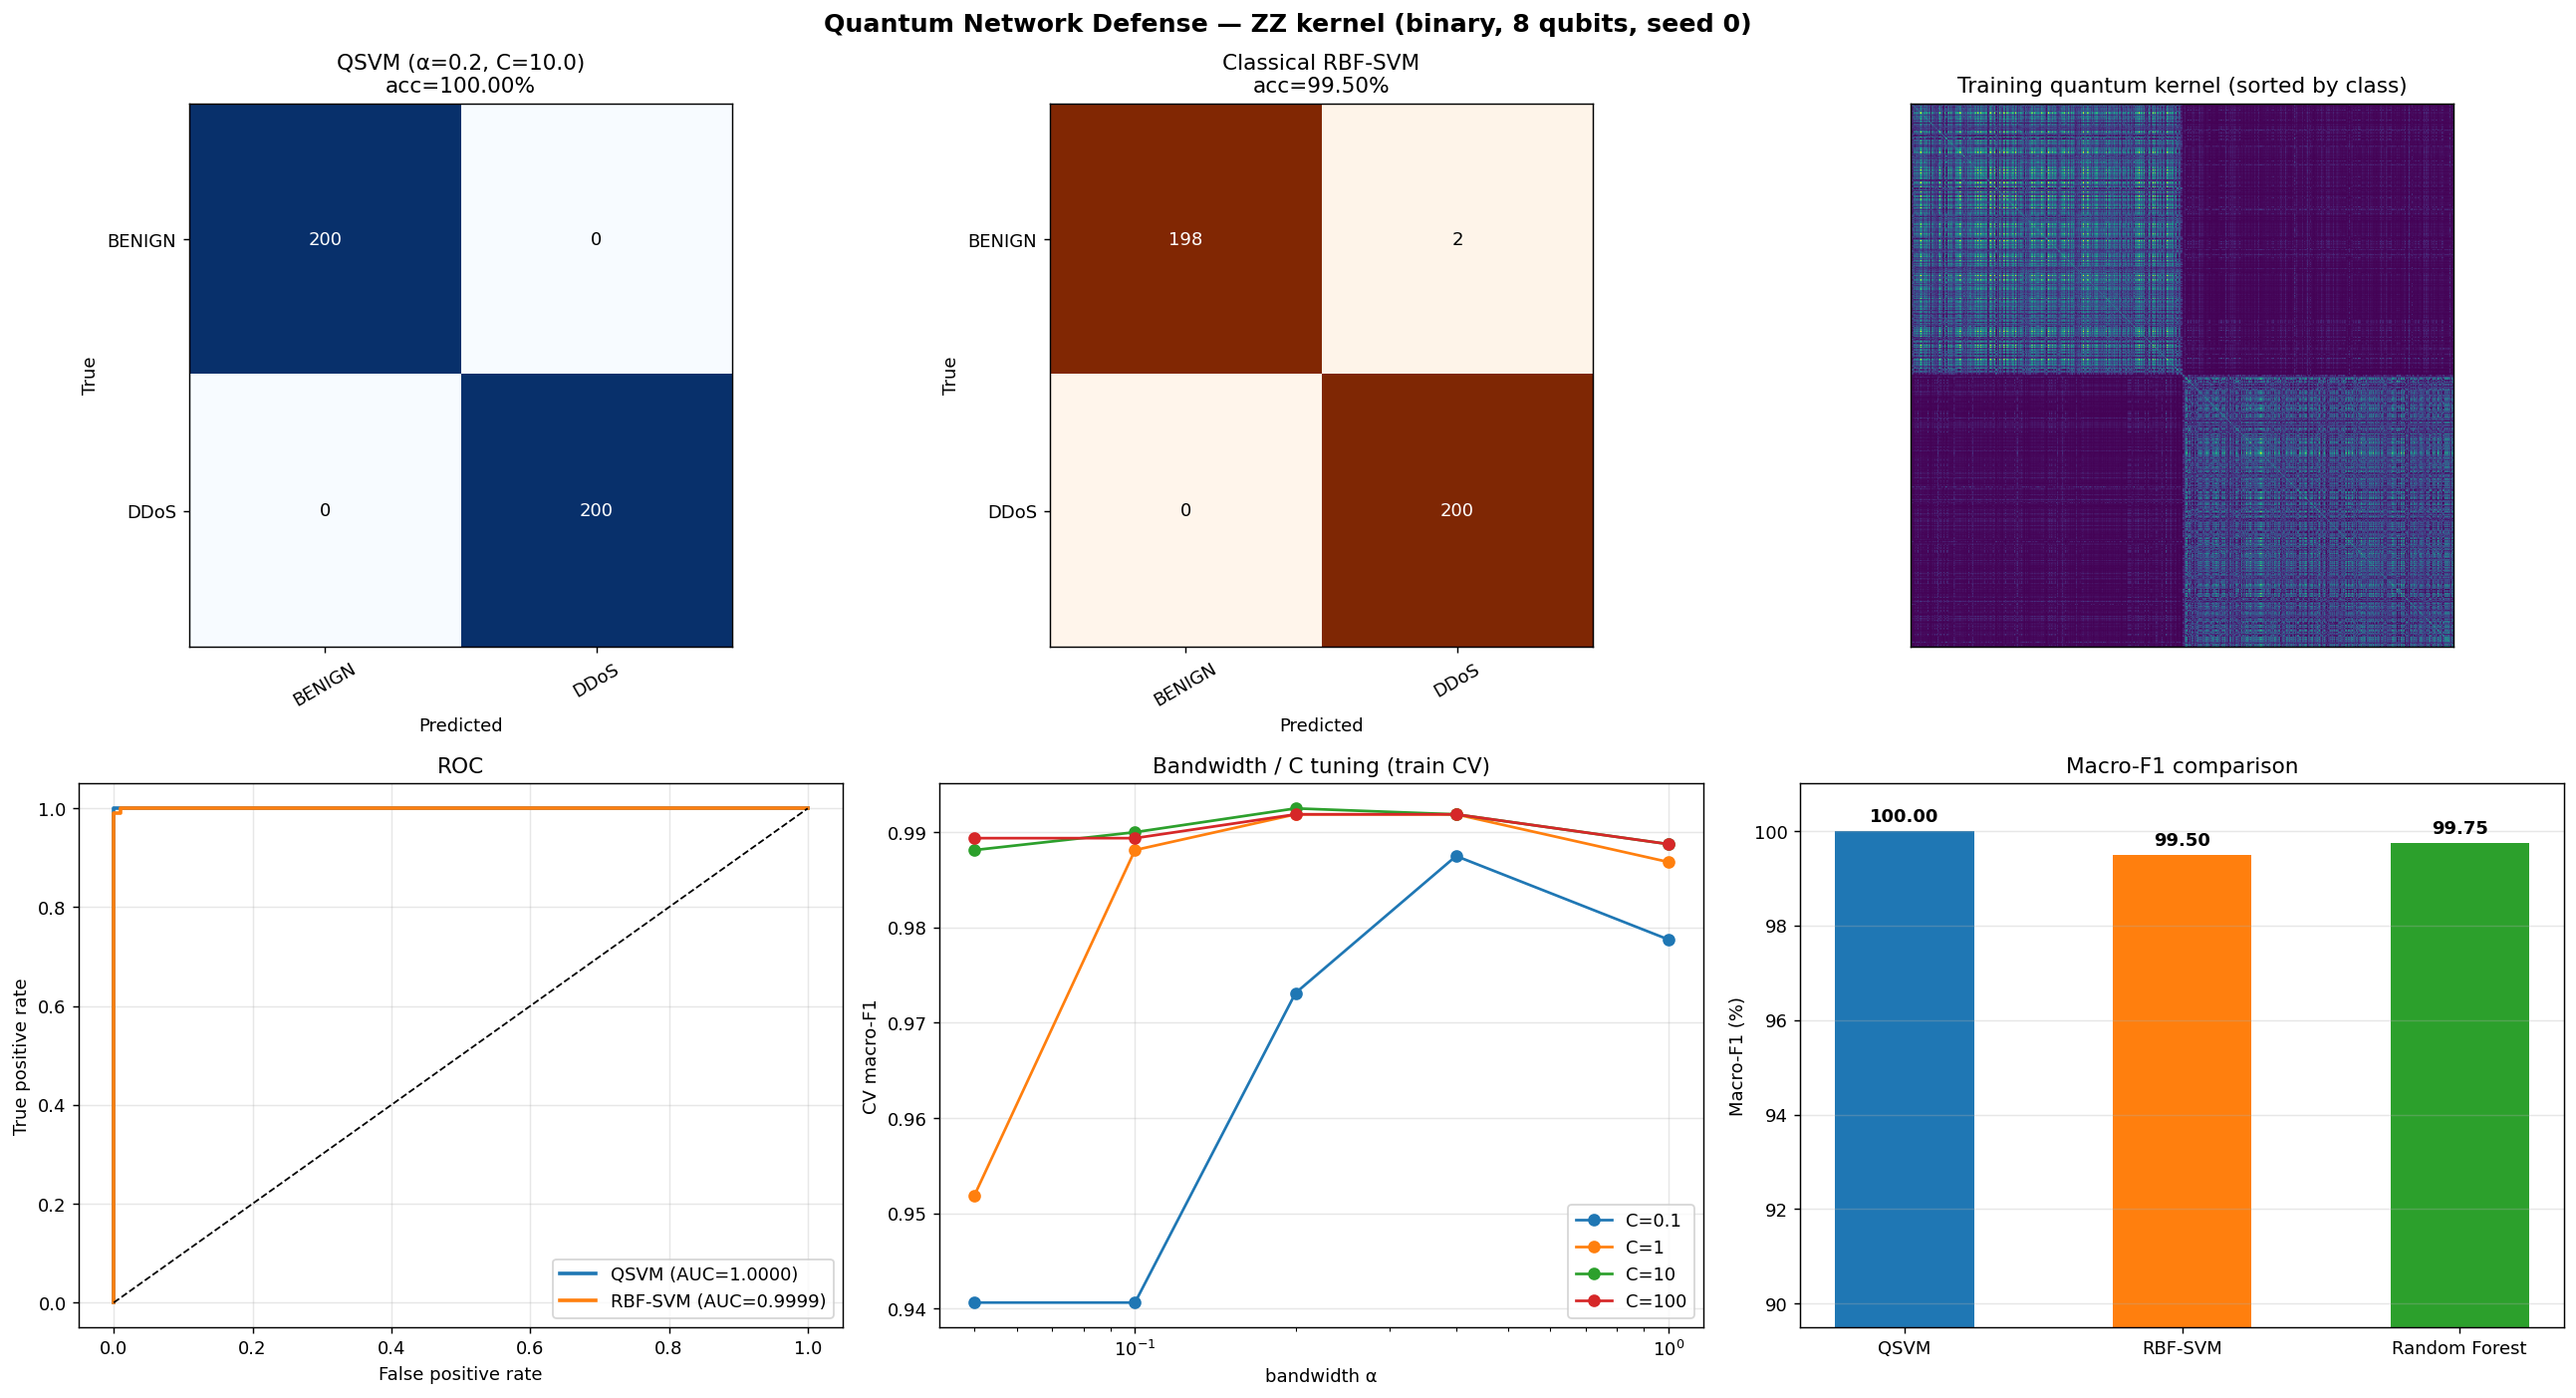
\includegraphics[width=\linewidth]{figures/run_binary.png}
\caption{Per-run figure written by \code{main.py} (binary task, ZZ map with 8 qubits and 2 reps,
improved protocol, seed 0). Top: QSVM and RBF confusion matrices, and the training quantum kernel
sorted by class (the block structure shows class-aware similarity). Bottom: ROC curves, the CV
tuning curves over $\alpha$ for each $C$, and macro-F1 of all models.}
\label{fig:runfig}
\end{figure}

\section{Results}
\label{sec:results}

\paragraph{Protocol.} Every number below is produced by \code{benchmark.py} and turned into tables
and figures by \code{make\_figures.py}. The headline and ablation experiments use 5 seeds
(0--4); all other sweeps use 3 seeds (0--2). Each seed redraws the balanced sample, the
80/20 stratified split, the preprocessing, the tuning and the test. With the default 2{,}000
samples the test set has 400 flows, so one flow is 0.25 accuracy points. ``Sig.'' is the number
of seeds in which the exact McNemar test (QSVM vs.\ RBF-SVM, same test flows) gives $p<0.05$.
Unless stated otherwise, the improved protocol is used: deduplication on the task label,
train-only preprocessing with the signed log transform, and 5-fold CV tuning of
$(\alpha, C)$ for the QSVM and $(C,\gamma)$ for the RBF-SVM with the same $C$ grid.

\subsection{Headline: the same circuits under the original and the improved protocol}

Table~\ref{tab:headline} runs the paper's three methods (the ZZ entangling map with the
paper's circuit settings, the separable $R_x$ map and its 1024-shot version) under both
protocols, plus a 16-qubit, 2-repetition ZZ circuit. Figure~\ref{fig:headline} shows the same
data.

\begin{table}[H]
\centering\small
\caption{Test accuracy (\%) and QSVM macro-F1 (\%), mean $\pm$ std over 5 seeds. ``Legacy'' is
the original protocol (\code{--legacy}); ``improved'' is the corrected one. ZZ uses the paper's
settings: 8 qubits / 2 reps (binary) and 16 qubits / 1 rep (multiclass). $R_x$ uses 16 qubits.}
\label{tab:headline}
\resizebox{\linewidth}{!}{%
\begin{tabular}{lllcccc}
\toprule
Task & Method & Protocol & QSVM acc. & RBF-SVM acc. & QSVM macro-F1 & Sig. \\
\midrule
binary & ZZ entangling (paper circuit) & legacy & 99.50 $\pm$ 0.32 & 97.35 $\pm$ 0.25 & 99.50 $\pm$ 0.32 & 5/5 \\
binary & ZZ entangling (paper circuit) & improved & 99.60 $\pm$ 0.41 & 99.55 $\pm$ 0.29 & 99.60 $\pm$ 0.41 & 0/5 \\
binary & Analytical $R_x$ (separable) & legacy & 98.35 $\pm$ 0.12 & 98.60 $\pm$ 0.41 & 98.35 $\pm$ 0.12 & 0/5 \\
binary & Analytical $R_x$ (separable) & improved & 99.50 $\pm$ 0.32 & 99.50 $\pm$ 0.27 & 99.50 $\pm$ 0.32 & 0/5 \\
binary & Sampling, 1024 shots ($R_x$) & legacy & 98.30 $\pm$ 0.10 & 98.60 $\pm$ 0.41 & 98.30 $\pm$ 0.10 & 0/5 \\
binary & Sampling, 1024 shots ($R_x$) & improved & 99.30 $\pm$ 0.62 & 99.50 $\pm$ 0.27 & 99.30 $\pm$ 0.62 & 0/5 \\
binary & ZZ, 16 qubits, 2 reps & improved & 99.60 $\pm$ 0.25 & 99.50 $\pm$ 0.27 & 99.60 $\pm$ 0.25 & 0/5 \\
\midrule
multiclass & ZZ entangling (paper circuit) & legacy & 95.70 $\pm$ 0.56 & 88.85 $\pm$ 1.12 & 95.68 $\pm$ 0.59 & 5/5 \\
multiclass & ZZ entangling (paper circuit) & improved & 90.85 $\pm$ 0.85 & 91.05 $\pm$ 0.95 & 90.85 $\pm$ 0.86 & 0/5 \\
multiclass & Analytical $R_x$ (separable) & legacy & 91.70 $\pm$ 2.54 & 88.85 $\pm$ 1.12 & 91.60 $\pm$ 2.55 & 2/5 \\
multiclass & Analytical $R_x$ (separable) & improved & 91.05 $\pm$ 0.24 & 91.05 $\pm$ 0.95 & 91.10 $\pm$ 0.22 & 0/5 \\
multiclass & Sampling, 1024 shots ($R_x$) & legacy & 91.35 $\pm$ 1.30 & 88.85 $\pm$ 1.12 & 91.27 $\pm$ 1.32 & 2/5 \\
multiclass & Sampling, 1024 shots ($R_x$) & improved & 88.10 $\pm$ 0.41 & 91.05 $\pm$ 0.95 & 88.16 $\pm$ 0.37 & 2/5 \\
multiclass & ZZ, 16 qubits, 2 reps & improved & 91.20 $\pm$ 0.84 & 91.05 $\pm$ 0.95 & 91.22 $\pm$ 0.86 & 0/5 \\

\bottomrule
\end{tabular}}
\end{table}

\begin{figure}[H]
\centering
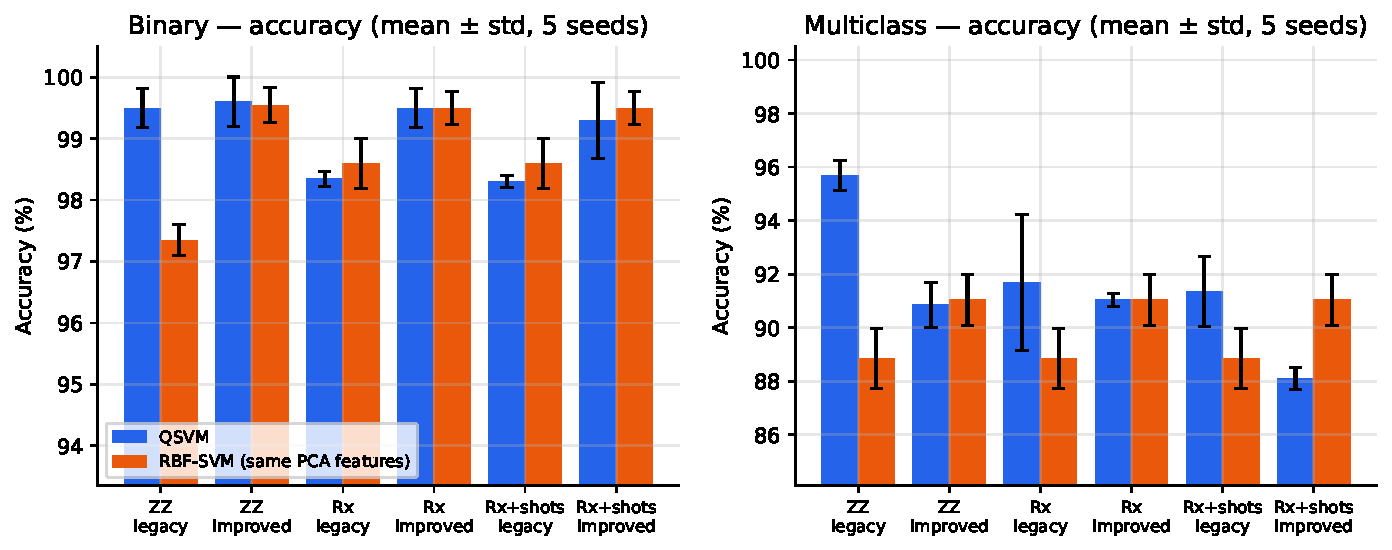
\includegraphics[width=\linewidth]{figures/headline.pdf}
\caption{Accuracy of the QSVM (blue) and the RBF-SVM on the same PCA features (orange) under
both protocols. Error bars: standard deviation over 5 seeds.}
\label{fig:headline}
\end{figure}

\paragraph{The original protocol reproduces the paper's pattern.} Under \code{--legacy} the ZZ
QSVM beats the RBF-SVM by $+2.15$ points (binary) and $+6.85$ points (multiclass), significant in
5/5 seeds both times. Summed over the five seeds, the QSVM is right where the RBF-SVM is wrong on
46 binary flows and the reverse happens on 3; in multiclass the counts are 172 and 35. The
paper's observation is therefore real \emph{under its protocol}.

\paragraph{The improved protocol removes the gap.} With the same circuits, the differences shrink
to $+0.05$ (binary) and $-0.20$ points (multiclass), and no seed is significant. Pooled over the
seeds, the discordant counts are 2 vs.\ 1 (binary) and 19 vs.\ 23 (multiclass). The QSVM did not
become worse in binary mode (99.50\% $\to$ 99.60\%); the RBF-SVM became much better
(97.35\% $\to$ 99.55\%; multiclass 88.85\% $\to$ 91.05\%). The same holds for the 16-qubit,
2-repetition circuit (99.60 vs.\ 99.50; 91.20 vs.\ 91.05) and for the separable $R_x$ kernel,
which ties the RBF-SVM exactly in both tasks.

\paragraph{Shot noise.} In binary mode the 1024-shot $R_x$ kernel is within noise of the exact
one. In multiclass mode it costs about 3 points (88.10\% vs.\ 91.05\% exact), and the RBF-SVM is
significantly better in 2/5 seeds. Section~\ref{sec:res-shots} explains why this happens at 16
qubits but not at 8.

\subsection{Ablation: which fix changes what}

Table~\ref{tab:ablation} and Figure~\ref{fig:ablation} add the fixes one at a time to the ZZ
pipeline with the paper's circuit settings, starting from the original protocol.

\begin{table}[H]
\centering\small
\caption{Cumulative ablation (5 seeds). ``Overlap'' is the fraction of test flows with an exact
copy in the training set. Gap = QSVM $-$ RBF-SVM accuracy in points.}
\label{tab:ablation}
\begin{tabular}{llccccc}
\toprule
Task & Step & Overlap & QSVM acc. & RBF-SVM acc. & Gap & Sig. \\
\midrule
binary & Original protocol & 28.4\% & 99.50 $\pm$ 0.32 & 97.35 $\pm$ 0.25 & +2.15 & 5/5 \\
binary & + remove duplicates & 0.0\% & 98.85 $\pm$ 0.49 & 96.15 $\pm$ 0.51 & +2.70 & 4/5 \\
binary & + train-only scaling & 0.0\% & 98.65 $\pm$ 0.34 & 96.40 $\pm$ 0.89 & +2.25 & 3/5 \\
binary & + log transform & 0.0\% & 99.15 $\pm$ 0.46 & 99.40 $\pm$ 0.68 & -0.25 & 0/5 \\
binary & + CV tuning ($\alpha$, $C$, $\gamma$) & 0.0\% & 99.60 $\pm$ 0.41 & 99.55 $\pm$ 0.29 & +0.05 & 0/5 \\
\midrule
multiclass & Original protocol & 48.6\% & 95.70 $\pm$ 0.56 & 88.85 $\pm$ 1.12 & +6.85 & 5/5 \\
multiclass & + remove duplicates & 0.8\% & 89.20 $\pm$ 1.02 & 87.55 $\pm$ 1.44 & +1.65 & 2/5 \\
multiclass & + train-only scaling & 0.8\% & 88.40 $\pm$ 1.22 & 87.35 $\pm$ 1.45 & +1.05 & 2/5 \\
multiclass & + log transform & 0.8\% & 91.40 $\pm$ 0.78 & 90.20 $\pm$ 0.58 & +1.20 & 0/5 \\
multiclass & + CV tuning ($\alpha$, $C$, $\gamma$) & 0.8\% & 90.85 $\pm$ 0.85 & 91.05 $\pm$ 0.95 & -0.20 & 0/5 \\

\bottomrule
\end{tabular}
\end{table}

\begin{figure}[H]
\centering
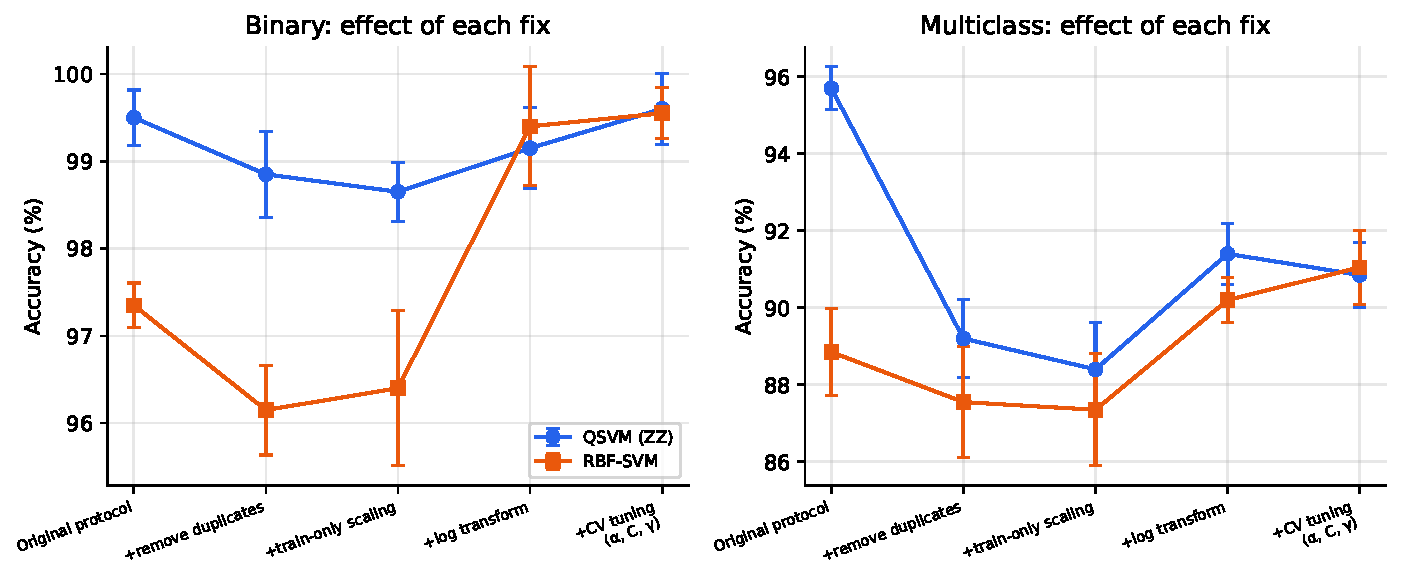
\includegraphics[width=0.95\linewidth]{figures/ablation.pdf}
\caption{Effect of each fix on QSVM and RBF-SVM accuracy (mean $\pm$ std, 5 seeds).}
\label{fig:ablation}
\end{figure}

\begin{itemize}
\item \textbf{Removing duplicates} is the largest single effect in multiclass mode. The QSVM
      loses 6.5 points (95.70\% $\to$ 89.20\%) and the gap shrinks from $+6.85$ to $+1.65$. The
      QSVM profited more from duplicates than the RBF-SVM: with $\alpha=1$ its kernel is close to
      the identity, so a test flow with a training twin gets $K=1$ to that twin and almost 0 to
      everything else, which is pure memorisation. In binary mode the overlap was smaller (28\%)
      and both models lose 0.65--1.2 points.
\item \textbf{Train-only scaling} changes little on its own ($\le$0.8 points). It is a
      correctness fix, not a performance one.
\item \textbf{The log transform} closes the binary gap. The RBF-SVM jumps by 3.0 points
      (96.40\% $\to$ 99.40\%) and the gap goes from $+2.25$ to $-0.25$. Under linear min--max
      scaling the heavy-tailed features squeeze most flows into a small corner of each PCA
      component (Figure~\ref{fig:skew}), and the RBF-SVM with a default $\gamma$ suffers from this
      much more than the QSVM. Part of the original ``advantage'' was therefore an encoding
      artefact that hurt the baseline.
\item \textbf{CV tuning} gives the last few tenths of a point and removes the remaining multiclass
      gap ($+1.20 \to -0.20$).
\end{itemize}

\subsection{All metrics for the improved ZZ pipeline}

\begin{table}[H]
\centering\small
\caption{All metrics (\%), improved protocol, ZZ with the paper's circuit settings, 5 seeds.
FAR: benign flows flagged as attacks. DR: attack flows flagged as some attack.}
\label{tab:metrics}
\resizebox{\linewidth}{!}{%
\begin{tabular}{llccccccc}
\toprule
Task & Model & Accuracy & Bal.\ acc. & Macro-F1 & MCC & AUC & FAR & DR \\
\midrule
binary & QSVM ZZ (tuned) & 99.60 $\pm$ 0.41 & 99.60 $\pm$ 0.41 & 99.60 $\pm$ 0.41 & 99.20 $\pm$ 0.81 & 99.92 $\pm$ 0.15 & 0.30 $\pm$ 0.40 & 99.50 $\pm$ 0.63 \\
binary & RBF-SVM (tuned) & 99.55 $\pm$ 0.29 & 99.55 $\pm$ 0.29 & 99.55 $\pm$ 0.29 & 99.10 $\pm$ 0.58 & 99.92 $\pm$ 0.14 & 0.40 $\pm$ 0.37 & 99.50 $\pm$ 0.63 \\
binary & Random Forest & 99.70 $\pm$ 0.29 & 99.70 $\pm$ 0.29 & 99.70 $\pm$ 0.29 & 99.40 $\pm$ 0.58 & 99.99 $\pm$ 0.02 & 0.10 $\pm$ 0.20 & 99.50 $\pm$ 0.63 \\
\midrule
multiclass & QSVM ZZ (tuned) & 90.85 $\pm$ 0.85 & 90.86 $\pm$ 0.85 & 90.85 $\pm$ 0.86 & 89.05 $\pm$ 1.01 & 98.71 $\pm$ 0.15 & 1.79 $\pm$ 1.46 & 98.62 $\pm$ 0.73 \\
multiclass & RBF-SVM (tuned) & 91.05 $\pm$ 0.95 & 91.06 $\pm$ 0.95 & 91.07 $\pm$ 0.98 & 89.29 $\pm$ 1.14 & 98.73 $\pm$ 0.28 & 2.09 $\pm$ 2.02 & 98.98 $\pm$ 0.67 \\
multiclass & Random Forest & 93.10 $\pm$ 0.49 & 93.11 $\pm$ 0.49 & 93.11 $\pm$ 0.48 & 91.74 $\pm$ 0.58 & 99.03 $\pm$ 0.07 & 2.09 $\pm$ 1.52 & 99.46 $\pm$ 0.29 \\

\bottomrule
\end{tabular}}
\end{table}

Table~\ref{tab:metrics} confirms the headline with every metric: the QSVM and the RBF-SVM are
within one standard deviation of each other on accuracy, balanced accuracy, macro-F1, MCC, AUC,
false-alarm rate and detection rate. The Random Forest on all 49 raw features is the best model
in both tasks (99.70\% binary, 93.10\% multiclass). The kernel models only see at most 16 PCA
components, and that compression has a cost.

\paragraph{Where the multiclass errors are.} Summed over the five seeds, the QSVM's per-class
recall is BENIGN 98.2\%, UDP 95.5\%, Syn 92.5\%, LDAP 89.2\%, MSSQL 87.4\% and Portmap 82.3\%.
The RBF-SVM's recalls are within 1 point of these for every class. Almost all errors are
confusions between the three reflection attacks (LDAP $\leftrightarrow$ MSSQL $\leftrightarrow$
Portmap), plus Portmap flows predicted as BENIGN or Syn. These are the classes whose flows are
70--94\% duplicates in the raw file, so they are the ones that looked easiest under the original
protocol. The Random Forest gains most on MSSQL (+4.5), Portmap (+4.5) and UDP (+3.3).

\subsection{Bandwidth $\alpha$}

Table~\ref{tab:bandwidth} and Figure~\ref{fig:bandwidth} fix $\alpha$ (tuning only $C$) for the
ZZ map with 2 repetitions at 8 and 16 qubits.

\begin{figure}[H]
\centering
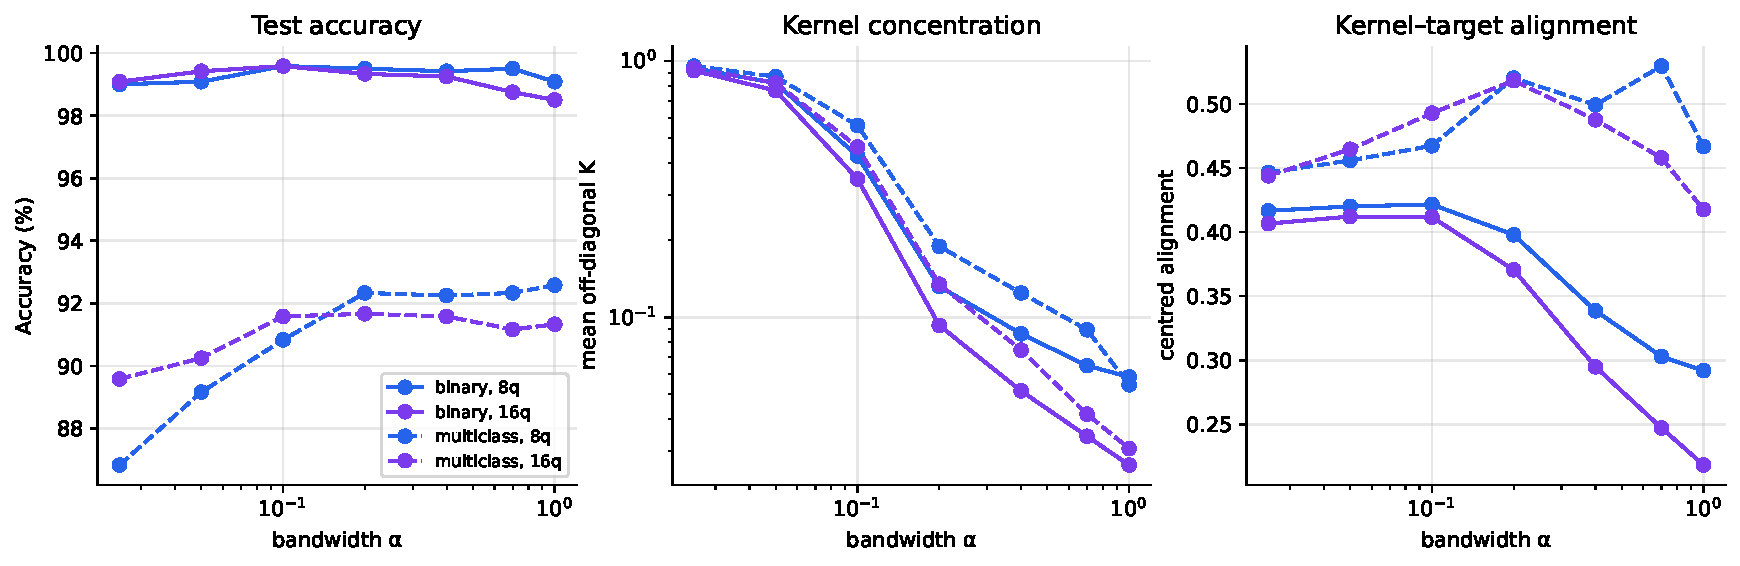
\includegraphics[width=\linewidth]{figures/bandwidth.pdf}
\caption{Test accuracy, mean off-diagonal kernel value and centred kernel--target alignment as
functions of $\alpha$ (ZZ map, 2 reps, 3 seeds).}
\label{fig:bandwidth}
\end{figure}

\begin{table}[H]
\centering\small
\caption{Bandwidth sweep (3 seeds): QSVM accuracy (\%), mean off-diagonal training kernel value,
and centred kernel--target alignment.}
\label{tab:bandwidth}
\begin{tabular}{lcccccc}
\toprule
Task & Qubits & $\alpha$ & QSVM acc. & Mean off-diag.\ $K$ & Alignment \\
\midrule
binary & 8 & 0.025 & 99.00 & 9.38e-01 & 0.417 \\
binary & 8 & 0.05 & 99.08 & 8.19e-01 & 0.420 \\
binary & 8 & 0.1 & 99.58 & 4.26e-01 & 0.422 \\
binary & 8 & 0.2 & 99.50 & 1.32e-01 & 0.398 \\
binary & 8 & 0.4 & 99.42 & 8.62e-02 & 0.339 \\
binary & 8 & 0.7 & 99.50 & 6.47e-02 & 0.303 \\
binary & 8 & 1 & 99.08 & 5.85e-02 & 0.292 \\
binary & 16 & 0.025 & 99.08 & 9.17e-01 & 0.407 \\
binary & 16 & 0.05 & 99.42 & 7.66e-01 & 0.412 \\
binary & 16 & 0.1 & 99.58 & 3.46e-01 & 0.412 \\
binary & 16 & 0.2 & 99.33 & 9.29e-02 & 0.371 \\
binary & 16 & 0.4 & 99.25 & 5.16e-02 & 0.295 \\
binary & 16 & 0.7 & 98.75 & 3.43e-02 & 0.247 \\
binary & 16 & 1 & 98.50 & 2.65e-02 & 0.218 \\
multiclass & 8 & 0.025 & 86.83 & 9.56e-01 & 0.446 \\
multiclass & 8 & 0.05 & 89.17 & 8.69e-01 & 0.456 \\
multiclass & 8 & 0.1 & 90.83 & 5.60e-01 & 0.467 \\
multiclass & 8 & 0.2 & 92.33 & 1.89e-01 & 0.520 \\
multiclass & 8 & 0.4 & 92.25 & 1.24e-01 & 0.499 \\
multiclass & 8 & 0.7 & 92.33 & 8.93e-02 & 0.530 \\
multiclass & 8 & 1 & 92.58 & 5.45e-02 & 0.467 \\
multiclass & 16 & 0.025 & 89.58 & 9.37e-01 & 0.444 \\
multiclass & 16 & 0.05 & 90.25 & 8.20e-01 & 0.465 \\
multiclass & 16 & 0.1 & 91.58 & 4.62e-01 & 0.493 \\
multiclass & 16 & 0.2 & 91.67 & 1.34e-01 & 0.518 \\
multiclass & 16 & 0.4 & 91.58 & 7.45e-02 & 0.488 \\
multiclass & 16 & 0.7 & 91.17 & 4.19e-02 & 0.458 \\
multiclass & 16 & 1 & 91.33 & 3.07e-02 & 0.418 \\

\bottomrule
\end{tabular}
\end{table}

\begin{itemize}
\item The mean off-diagonal kernel value falls by more than an order of magnitude from
      $\alpha=0.025$ to $\alpha=1$ (e.g.\ 0.92 $\to$ 0.027 at 16 qubits, binary). This is the
      concentration effect of Section~\ref{sec:conc}, and it is stronger at 16 qubits than at 8.
\item At 16 qubits, accuracy peaks at $\alpha\approx0.1$--0.2 and falls at $\alpha=1$ (binary
      99.58\% $\to$ 98.50\%), and alignment falls with it (0.41 $\to$ 0.22). At 8 qubits the
      kernel concentrates less, so the curve is flatter. Without a bandwidth, the paper's
      16-qubit circuit sits in the worst part of the curve.
\item Very small $\alpha$ also hurts, especially in multiclass mode (86.8\% at 8 qubits,
      $\alpha=0.025$): the kernel approaches the constant 1 and the classes are no longer
      separated.
\item In binary mode, alignment and accuracy peak at the same $\alpha$ ($\approx0.1$); in
      multiclass mode they peak at roughly similar values. The cheap alignment diagnostic (no SVM
      training needed) is therefore a rough guide for choosing $\alpha$, but not a substitute
      for CV.
\end{itemize}

\subsection{Number of qubits}

\begin{figure}[H]
\centering
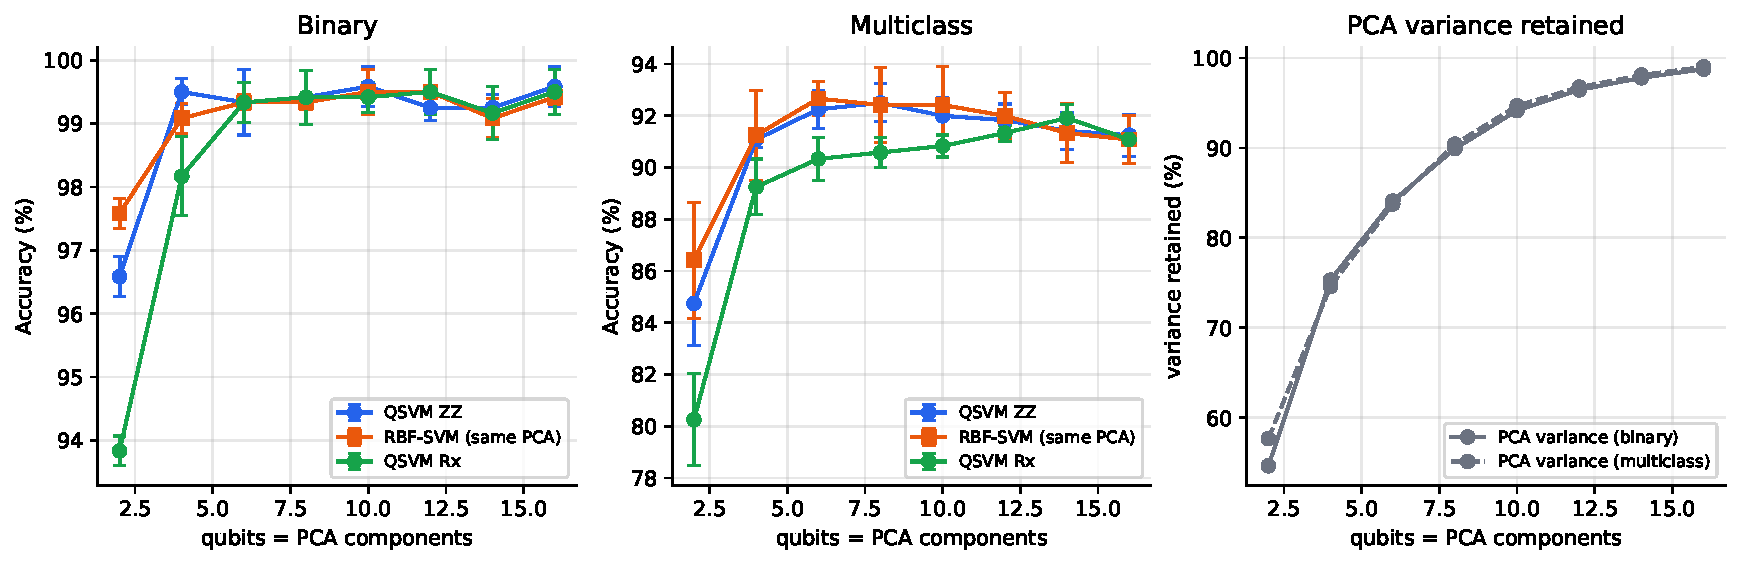
\includegraphics[width=\linewidth]{figures/qubits.pdf}
\caption{Accuracy vs.\ number of qubits (= PCA components) for the ZZ and $R_x$ QSVMs and the
RBF-SVM on the same components, and the PCA variance retained (3 seeds).}
\label{fig:qubits}
\end{figure}

\begin{table}[H]
\centering\small
\caption{Qubit sweep for the ZZ map (2 reps, 3 seeds): PCA variance retained (\%), accuracy (\%),
mean tuned $\alpha$ and geometric difference $g$ against the tuned RBF kernel
($\sqrt{N}=20$).}
\label{tab:qubits}
\begin{tabular}{lcccccc}
\toprule
Task & Qubits & PCA var. & QSVM ZZ & RBF-SVM & Mean $\alpha$ & $g$ \\
\midrule
binary & 2 & 54.6 & 96.58 & 97.58 & 1.000 & 39.36 \\
binary & 4 & 75.3 & 99.50 & 99.08 & 0.333 & 10.26 \\
binary & 6 & 84.1 & 99.33 & 99.33 & 0.400 & 3.75 \\
binary & 8 & 89.9 & 99.42 & 99.33 & 0.333 & 14.49 \\
binary & 10 & 94.2 & 99.58 & 99.50 & 0.233 & 10.14 \\
binary & 12 & 96.4 & 99.25 & 99.50 & 0.133 & 14.06 \\
binary & 14 & 97.8 & 99.25 & 99.08 & 0.133 & 8.97 \\
binary & 16 & 98.8 & 99.58 & 99.42 & 0.100 & 2.22 \\
multiclass & 2 & 57.7 & 84.75 & 86.42 & 1.000 & 31.05 \\
multiclass & 4 & 74.6 & 91.08 & 91.25 & 0.800 & 32.40 \\
multiclass & 6 & 83.7 & 92.25 & 92.67 & 0.800 & 9.77 \\
multiclass & 8 & 90.4 & 92.50 & 92.42 & 0.800 & 17.52 \\
multiclass & 10 & 94.7 & 92.00 & 92.42 & 0.333 & 3.00 \\
multiclass & 12 & 96.8 & 91.83 & 92.00 & 0.233 & 7.86 \\
multiclass & 14 & 98.1 & 91.42 & 91.33 & 0.333 & 2.50 \\
multiclass & 16 & 99.0 & 91.25 & 91.08 & 0.333 & 3.94 \\

\bottomrule
\end{tabular}
\end{table}

Accuracy saturates early: at 4 qubits the binary task is already at 99.5\%, and multiclass
accuracy stops improving at 6--8 qubits (84--90\% PCA variance). From 4 qubits on, the QSVM and
the RBF-SVM are within 0.5 points of each other at every width; only at 2 qubits is the RBF-SVM
1--1.7 points ahead. As the circuit gets wider, the tuned $\alpha$ falls (from 1.0 at 2 qubits
to 0.1--0.33 at 12--16 qubits), which is the tuning compensating for concentration. Adding qubits makes the Hilbert space exponentially larger, but
that does not show up in accuracy.

\subsection{Shot noise}
\label{sec:res-shots}

\begin{figure}[H]
\centering
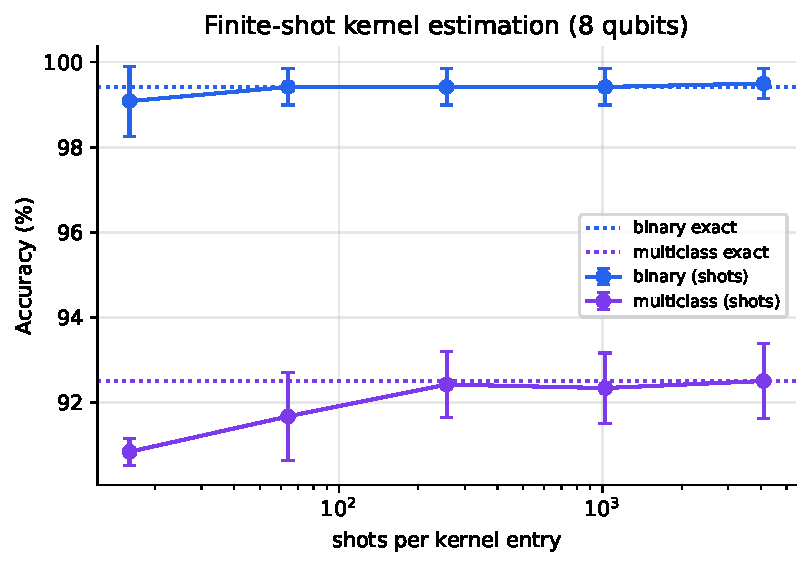
\includegraphics[width=0.6\linewidth]{figures/shots.pdf}
\caption{QSVM accuracy vs.\ shots per kernel entry (ZZ, 8 qubits, 2 reps, 3 seeds). Dotted lines:
exact kernel.}
\label{fig:shots}
\end{figure}

\begin{table}[H]
\centering\small
\caption{Shot sweep, ZZ map, 8 qubits (3 seeds): accuracy (\%) and mean tuned $\alpha$.}
\label{tab:shots}
\begin{tabular}{lccc}
\toprule
Task & Shots & QSVM acc. & Mean $\alpha$ \\
\midrule
binary & 16 & 99.08 $\pm$ 0.82 & 0.533 \\
binary & 64 & 99.42 $\pm$ 0.42 & 0.400 \\
binary & 256 & 99.42 $\pm$ 0.42 & 0.333 \\
binary & 1024 & 99.42 $\pm$ 0.42 & 0.267 \\
binary & 4096 & 99.50 $\pm$ 0.35 & 0.267 \\
binary & exact & 99.42 $\pm$ 0.42 & 0.333 \\
multiclass & 16 & 90.83 $\pm$ 0.31 & 1.000 \\
multiclass & 64 & 91.67 $\pm$ 1.03 & 1.000 \\
multiclass & 256 & 92.42 $\pm$ 0.77 & 1.000 \\
multiclass & 1024 & 92.33 $\pm$ 0.82 & 1.000 \\
multiclass & 4096 & 92.50 $\pm$ 0.89 & 0.800 \\
multiclass & exact & 92.50 $\pm$ 0.74 & 0.800 \\

\bottomrule
\end{tabular}
\end{table}

At 8 qubits, 256 shots per entry already match the exact kernel in both tasks, and even 16
shots cost only 0.3 (binary) and 1.7 points (multiclass). The tuned $\alpha$ moves to larger
values as the shot count falls (binary: 0.27 at 1024--4096 shots, 0.53 at 16). A likely reason
is that larger $\alpha$ pushes most kernel values towards 0, where the binomial variance
$K(1-K)/s$ is small, so CV picks a bandwidth that limits the noise.

The 16-qubit $R_x$ result in Table~\ref{tab:headline} is different: there, 1024 shots cost 3
points in multiclass mode, while in binary mode they cost nothing. With 1024 shots each entry has
a standard deviation of up to $\sqrt{0.25/1024}\approx0.016$. The binary classes are far apart
in kernel space, but the three reflection attacks are separated by small kernel differences that
are apparently of the same order. We have not isolated why the 8-qubit ZZ kernel is robust and
the 16-qubit $R_x$ kernel is not. The practical lesson is that the shot budget needed depends on
the circuit and the task, and has to be measured before trusting a hardware result.

\paragraph{Projecting the noisy kernel onto the PSD cone does not help.} An estimated Gram matrix
is not positive semi-definite. On 1{,}600 multiclass training flows (16 qubits, $R_x$, 1024
shots), the negative eigenvalues sum to between $-83$ and $-319$ depending on $\alpha$, so the
SVM dual is no longer convex. The standard remedy is to clip the negative eigenvalues of the
training kernel to zero~\cite{hubregtsen2022}, available as \code{--psd}. On the multiclass
headline it made results worse in 5/5 seeds (88.10\% $\to$ 84.65\%). Clipping changes only the
training kernel, while the test kernel keeps its noise, so the two no longer describe the same
geometry. The option is therefore off by default.

\subsection{Circuit architecture and feature set}

\begin{table}[H]
\centering\small
\caption{ZZ QSVM accuracy (\%) by number of repetitions and entanglement topology (8 qubits,
3 seeds).}
\label{tab:arch}
\begin{tabular}{llccc}
\toprule
Task & Reps & Linear & Circular & Full \\
\midrule
binary & 1 & 99.25 $\pm$ 0.20 & 99.25 $\pm$ 0.20 & 99.25 $\pm$ 0.41 \\
binary & 2 & 99.42 $\pm$ 0.42 & 99.50 $\pm$ 0.35 & 99.33 $\pm$ 0.24 \\
binary & 3 & 99.42 $\pm$ 0.42 & 99.17 $\pm$ 0.24 & 99.42 $\pm$ 0.12 \\
\midrule
multiclass & 1 & 92.58 $\pm$ 0.66 & 92.50 $\pm$ 0.71 & 92.50 $\pm$ 0.54 \\
multiclass & 2 & 92.50 $\pm$ 0.74 & 92.58 $\pm$ 0.82 & 92.00 $\pm$ 0.35 \\
multiclass & 3 & 92.42 $\pm$ 1.45 & 92.75 $\pm$ 0.89 & 91.92 $\pm$ 0.12 \\

\bottomrule
\end{tabular}
\end{table}

No architecture stands out (Table~\ref{tab:arch}). All nine combinations of 1--3 repetitions and
linear, circular or full entanglement are within 0.35 points of each other in binary mode and
0.85 points in multiclass mode, which is within one standard deviation. More entanglement or more
repetitions, which make the kernel harder to simulate classically, do not make it more accurate
here.

\begin{table}[H]
\centering\small
\caption{Feature set (8 qubits, 3 seeds): accuracy (\%).}
\label{tab:features}
\begin{tabular}{llccc}
\toprule
Task & Feature set & QSVM ZZ & RBF-SVM & Random Forest \\
\midrule
binary & paper (61 listed, 49 non-constant) & 99.42 $\pm$ 0.42 & 99.33 $\pm$ 0.12 & 99.50 $\pm$ 0.20 \\
binary & all numeric CICFlowMeter columns & 99.42 $\pm$ 0.31 & 99.50 $\pm$ 0.54 & 99.67 $\pm$ 0.12 \\
multiclass & paper (61 listed, 49 non-constant) & 92.50 $\pm$ 0.74 & 92.42 $\pm$ 1.43 & 93.17 $\pm$ 0.59 \\
multiclass & all numeric CICFlowMeter columns & 93.92 $\pm$ 0.72 & 94.25 $\pm$ 0.35 & 94.67 $\pm$ 0.24 \\

\bottomrule
\end{tabular}
\end{table}

Using all 77 numeric CICFlowMeter columns instead of the paper's list (Table~\ref{tab:features})
adds 1.4--1.8 points in multiclass mode for \emph{every} model. The extra Subflow,
\code{Init\_Win\_bytes} and Active/Idle columns carry real information about the reflection
attacks. The gap between the models does not change.

\subsection{Learning curves}

\begin{figure}[H]
\centering
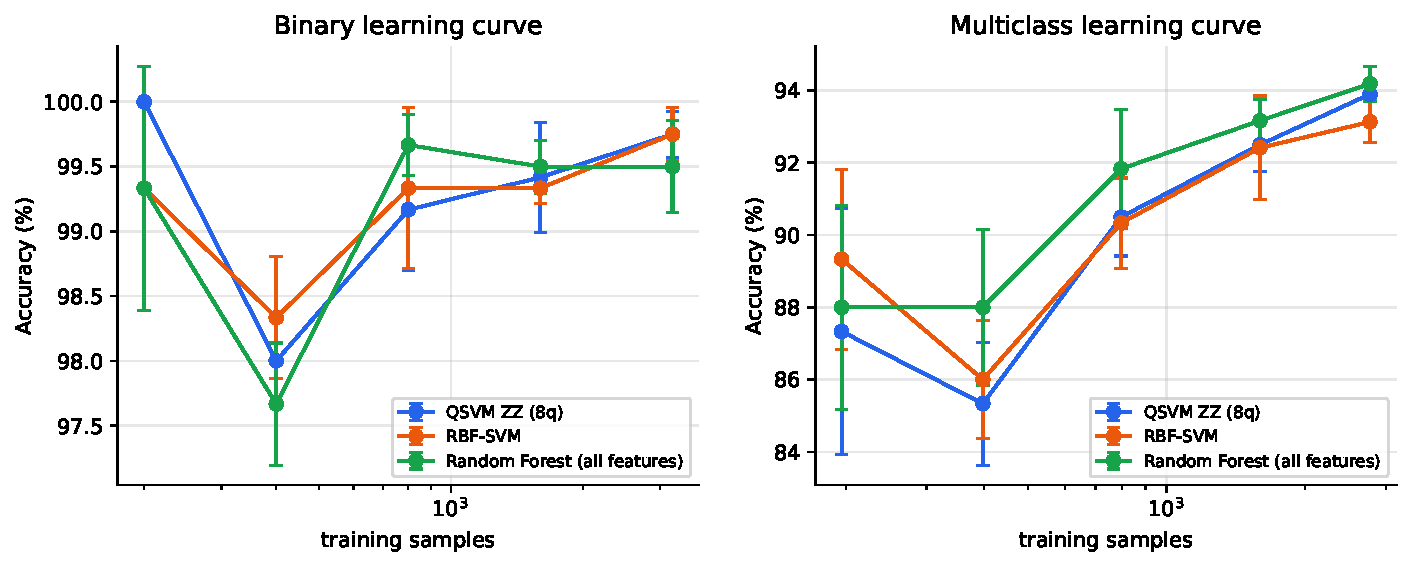
\includegraphics[width=0.95\linewidth]{figures/samples.pdf}
\caption{Accuracy vs.\ number of training flows (8 qubits, 3 seeds). In multiclass mode the
largest setting is capped at 2{,}774 training flows by the 578 unique LDAP flows.}
\label{fig:samples}
\end{figure}

The QSVM and RBF-SVM curves overlap at every size from 200 to 3{,}200 training flows
(Figure~\ref{fig:samples}). Neither model learns faster from few examples, which is sometimes
proposed as an advantage of quantum kernels. Multiclass accuracy is still rising at the largest
size (93.9\% QSVM, 93.1\% RBF-SVM, 94.2\% Random Forest), so more data would help all models, but
deduplication leaves only 578 LDAP flows in this file.

\subsection{Kernel diagnostics}

\begin{table}[H]
\centering\small
\caption{Kernel diagnostics on the training kernel (headline runs, mean over 5 seeds):
off-diagonal mean and standard deviation, centred alignment of the quantum and the tuned RBF
kernel, and the geometric difference $g(K_\text{RBF}\|K_Q)$ on 400 training flows.}
\label{tab:diag}
\resizebox{\linewidth}{!}{%
\begin{tabular}{llccccc}
\toprule
Task & Kernel & Off-diag.\ mean & Off-diag.\ std & Align.\ $K_Q$ & Align.\ $K_\text{RBF}$ & $g(K_\text{RBF}\|K_Q)$ \\
\midrule
binary & ZZ, original ($\alpha{=}1$) & 0.0781 & 0.239 & 0.297 & 0.233 & 65.74 (vs $\sqrt{N}$=20) \\
binary & ZZ, tuned $\alpha$ & 0.0971 & 0.249 & 0.353 & 0.348 & 10.85 (vs $\sqrt{N}$=20) \\
binary & ZZ 16q/2 reps, tuned $\alpha$ & 0.427 & 0.242 & 0.433 & 0.296 & 4.03 (vs $\sqrt{N}$=20) \\
binary & $R_x$, tuned $\alpha$ & 0.294 & 0.267 & 0.370 & 0.296 & 2.90 (vs $\sqrt{N}$=20) \\
\midrule
multiclass & ZZ, original ($\alpha{=}1$) & 0.0701 & 0.23 & 0.494 & 0.479 & 111.97 (vs $\sqrt{N}$=20) \\
multiclass & ZZ, tuned $\alpha$ & 0.0867 & 0.2 & 0.467 & 0.484 & 13.76 (vs $\sqrt{N}$=20) \\
multiclass & ZZ 16q/2 reps, tuned $\alpha$ & 0.084 & 0.218 & 0.487 & 0.484 & 9.19 (vs $\sqrt{N}$=20) \\
multiclass & $R_x$, tuned $\alpha$ & 0.379 & 0.287 & 0.516 & 0.484 & 3.08 (vs $\sqrt{N}$=20) \\

\bottomrule
\end{tabular}}
\end{table}

Table~\ref{tab:diag} explains the results.
\begin{itemize}
\item \textbf{Alignment.} With tuned $\alpha$, the quantum kernels are aligned with the labels about
      as well as the tuned RBF kernel is (binary 0.35--0.43 vs.\ 0.30--0.35; multiclass
      0.47--0.52 vs.\ 0.48). Equal alignment predicts equal accuracy, which is what we observe.
\item \textbf{Geometric difference.} For every tuned quantum kernel, $g$ is well below $\sqrt{N}=20$:
      2.9--3.1 for $R_x$, 4.0--9.2 for the 16-qubit ZZ map and 10.9--13.8 for the paper's ZZ
      settings. By Huang et al.~\cite{huang2021}, a classical kernel trained on the same data can then
      match the quantum kernel's predictions up to a small factor, so no large advantage is
      possible on this data, whatever the labels.
\item \textbf{The original protocol} gives very large $g$ (65.7 binary, 112.0 multiclass). This does
      \emph{not} indicate quantum power: under the original encoding the reference RBF kernel is
      itself badly scaled, and with $\alpha=1$ the quantum kernel is close to the identity, which
      makes \emph{any} smooth kernel look geometrically ``different''. A large $g$ is necessary for
      an advantage, not sufficient, and here the labels do not need the extra geometry.
\end{itemize}

\keybox{Summary of the results}{%
Under a leakage-free protocol with equal tuning, the ZZ quantum-kernel SVM and the classical
RBF-SVM are statistically indistinguishable on every metric, every circuit architecture, every
width from 4 to 16 qubits and every training-set size tested. The original advantages
(+2.15 and +6.85 points) come from duplicate leakage, which mostly helped the QSVM, and from a
linear encoding of heavy-tailed features, which mostly hurt the RBF baseline. A Random Forest
on all raw features is the best model in both tasks.}

\section{Discussion}
\label{sec:discussion}

\subsection{Does the quantum kernel help on this task?}
No, not on this data. Under the corrected protocol the ZZ quantum kernel matches a tuned
classical RBF kernel on the same PCA features. It does not beat it on any metric, circuit
architecture, qubit count or training-set size we tested, and a Random Forest on all raw
features beats both. This agrees with large systematic benchmarks of quantum models on classical
data~\cite{bowles2024}, which found that well-tuned classical baselines usually match or beat
them.

This is a negative result about \emph{this} dataset and feature map, not about quantum kernels in
general. The diagnostics show why it comes out this way:
\begin{enumerate}
\item \textbf{The problem is easy and low-dimensional.} Binary accuracy is 99.5\% with only 4 PCA
      components, and every model saturates at 6--8 components. There is little left for a more
      expressive kernel to find.
\item \textbf{The quantum kernel's geometry is classically reachable.} With tuned $\alpha$, the
      geometric difference to the RBF kernel is 3--14, well below $\sqrt{N}=20$. By
      Huang et al.~\cite{huang2021} a classical kernel can then reproduce the quantum kernel's
      predictions, so no large advantage is possible, whatever the labels.
\item \textbf{The useful regime of the ZZ map is the classical-looking one.} The tuning selects
      small $\alpha$ for the 16-qubit, 2-repetition circuit (0.05--0.4). There, the phases are small and the kernel behaves
      like a smooth, RBF-like similarity. The large-$\alpha$ regime, where the circuit is
      conjectured to be hard to simulate, is exactly where it concentrates and loses accuracy
      (Figure~\ref{fig:bandwidth}).
\item \textbf{Entanglement is not used.} The separable $R_x$ kernel, which is a classical closed-form
      expression, performs the same as the entangling ZZ kernel, and more repetitions or denser
      entanglement do not change accuracy (Table~\ref{tab:arch}).
\item \textbf{Flow statistics have no quantum structure.} Known quantum advantages for kernels use
      data whose labels are generated by a quantum process or encode a problem that is hard
      classically (e.g.\ discrete logarithms). CICFlowMeter statistics are classical summaries of
      packet counts and timings, and the ZZ feature map was not designed around them.
\end{enumerate}

\subsection{What went wrong in the original evaluation}
The original advantages were produced by the evaluation, not by the model. Ranked by effect:
\begin{enumerate}
\item \textbf{Duplicate leakage} (up to 49\% of test flows with a training twin). It inflated the
      QSVM more than the RBF-SVM: a nearly diagonal kernel memorises twins perfectly.
\item \textbf{Linear encoding of heavy-tailed features.} It hurt the RBF baseline much more than
      the QSVM (3 points in binary mode), creating most of the binary gap.
\item \textbf{Unequal tuning.} The RBF-SVM was run with default $C$ and $\gamma$. Comparing a
      configured model against a default one measures the configuration, not the model.
\item \textbf{Single small test sets.} The binary ZZ result rested on 165 test flows, where
      ``98.79\% vs.\ 96.97\%'' is 163 vs.\ 160 correct. No repetition or significance test was
      reported.
\end{enumerate}
These are general lessons for quantum-ML benchmarks on network data: deduplicate before
splitting, fit every transform on training data only, give the classical baseline the same
tuning budget, report several seeds with a paired test, and include a strong non-kernel
baseline.

\subsection{Threats to validity}
\begin{itemize}
\item \textbf{Simulation only.} All kernels are exact or binomially sampled statevector
      simulations. Hardware adds gate errors, decoherence and readout noise. The shot
      experiments model only statistical noise, and even that costs 3 points in the 16-qubit
      multiclass setting (Section~\ref{sec:res-shots}).
\item \textbf{One capture, contiguous slices.} Each class in \code{output.csv} is a contiguous slice of
      one capture day, in some cases spanning about a second. Random train/test splits within such
      a slice are easier than training on one day and testing on another. Cross-day or cross-dataset
      evaluation would be the stronger test, and it would make all models' accuracy lower.
\item \textbf{Balanced sampling.} Real traffic is heavily imbalanced, so the false-alarm rate would
      matter much more than accuracy. The FAR is reported, but not at a realistic base rate.
\item \textbf{Statistical power.} Each seed tests 400 flows, so per-seed McNemar tests only detect
      differences of roughly 2 points or more. Pooled over 5 seeds, the discordant counts are nearly
      balanced (2 vs.\ 1 binary, 19 vs.\ 23 multiclass), so a large hidden advantage is very
      unlikely, but differences below about 1 point cannot be ruled out.
\item \textbf{Shared preprocessing inside CV.} PCA and scaling are fitted once on the full
      training split, and the CV folds for tuning reuse that fit. The validation folds therefore
      contribute to the unsupervised preprocessing. This affects the QSVM and the RBF-SVM equally
      and does not touch the test set.
\item \textbf{Bandwidth grid boundary for $R_x$.} The tuned $\alpha$ of the $R_x$ kernel was 1.0, the
      top of the default grid, in all 10 headline runs. Rerunning the 16-qubit $R_x$ headline with
      $\alpha\in\{\dots,1.5,2,3\}$ selects $\alpha=1.5$--3 and raises accuracy slightly (binary
      99.50\% $\to$ 99.60\%, multiclass 91.05\% $\to$ 91.65\%), still with no significant seed
      against the RBF-SVM ($p\ge0.125$). The conclusion is unchanged, but the reported $R_x$
      numbers are slightly conservative. For the ZZ map the tuned $\alpha$ lies inside the grid.
\item \textbf{Ambiguous rows.} After deduplication, 177 multiclass rows (2 binary) share their
      feature vector with a row of a different class. They are kept as genuine ambiguity and
      cause the 0.8\% residual train/test overlap in multiclass mode.
\end{itemize}

\subsection{Future work}
\begin{enumerate}
\item \textbf{Harder data:} the 12 January capture day of CIC-DDoS2019 (DNS, NTP, SSDP, SNMP and
      other near-identical reflection attacks), cross-day train/test splits, and other datasets
      such as CICIDS2017 or UNSW-NB15. \code{--csv} already accepts any CICFlowMeter file.
\item \textbf{Trainable feature maps} that maximise kernel--target alignment
      (\code{evaluation.centered\_alignment} is already implemented).
\item \textbf{Projected quantum kernels}~\cite{huang2021}, which are less prone to concentration.
\item \textbf{Noise models and mitigation:} depolarising and readout noise on the Cirq backend,
      and noise-aware kernel post-processing that treats the training and test kernels
      consistently. Clipping only the training kernel's spectrum made results worse here.
\item \textbf{Hardware runs} of a subset of kernel entries using \code{build\_kernel\_circuit()}.
\item \textbf{Imbalanced evaluation:} train on balanced data, test at the natural class ratio, and
      report precision at a fixed false-alarm rate.
\end{enumerate}

\subsection{Conclusion}
The project now has a correct, fast and reproducible quantum-kernel pipeline. Kernels are
verified against Cirq, 16-qubit kernels take seconds instead of days, preprocessing is
leakage-free, tuning is equal, and the evaluation uses several seeds with significance tests.
With that pipeline, the reported quantum advantage on CIC-DDoS2019 does not survive. The ZZ
quantum kernel SVM is as good as, but not better than, a tuned classical RBF-SVM, and both are
slightly behind a Random Forest on all features. The tools built here (kernel diagnostics, the
geometric-difference test, the benchmark suite) can be used to test whether a quantum kernel helps
on harder data, and to find out quickly when it does not.

\appendix
\section{Command-line reference}
\label{app:cli}

\begin{table}[H]
\centering\small
\begin{tabularx}{\linewidth}{l l X}
\toprule
Option & Default & Meaning \\
\midrule
\code{--csv PATH} & \code{./output.csv} & input file (original) \\
\code{--samples N} & 2000 & total balanced sample size (original) \\
\code{--mode} & \code{binary} & \code{binary} or \code{multiclass} (original) \\
\code{--n-qubits n} & 16 & qubits = PCA components (original) \\
\code{--n-reps r} & 2 & feature-map repetitions (original) \\
\code{--sampling} & off & finite-shot kernel (original flag; now fast binomial emulation unless \code{--backend cirq}) \\
\code{--shots s} & 1024 & shots per kernel entry \\
\code{--kernel} & \code{zz} & \code{zz} (entangling) or \code{rx} (separable, paper Method 1) \\
\code{--entanglement} & \code{linear} & \code{linear}, \code{circular}, \code{full} \\
\code{--backend} & \code{fast} & \code{fast} (NumPy, exact) or \code{cirq} \\
\code{--alphas a...} & 0.05 0.1 0.2 0.4 1 & bandwidth grid for CV \\
\code{--Cs c...} & 0.1 1 10 100 & $C$ grid for CV (QSVM and RBF) \\
\code{--no-tune} & off & use \code{--alpha}/\code{--C} and an untuned RBF (\code{C=1, gamma='scale'}) \\
\code{--alpha a}, \code{--C c} & 1, 1 & fixed values when \code{--no-tune} \\
\code{--seeds k...} & 42 & one full run per seed; mean $\pm$ std reported \\
\code{--features} & \code{paper} & \code{paper} (61 listed columns) or \code{all} (77) \\
\code{--keep-duplicates} & off & do not deduplicate \\
\code{--no-log} & off & disable the signed log transform \\
\code{--legacy-scaling} & off & original preprocessing (global MinMax before split) \\
\code{--legacy} & off & = \code{--legacy-scaling --keep-duplicates --no-tune --alpha 1 --C 1} \\
\code{--extra-baselines} & off & also train a Random Forest on all raw features \\
\code{--out-dir DIR} & \code{outputs/<tag>} & where \code{results.json} and figures go \\
\code{--quiet} & off & suppress per-class reports and tuning logs \\
\bottomrule
\end{tabularx}
\end{table}

\section{File-by-file reference}
\label{app:files}
\begin{description}
\item[\code{data\_loader.py}] \code{load\_csv(csv\_path, mode, max\_samples, balance, dedup, feature\_set, seed, verbose)}
  $\to$ \code{(X\_raw, y, label\_names, info)}. Also \code{duplicate\_overlap(X\_train, X\_test)}.
  Constants \code{FEATURE\_COLS} (61 names), \code{META\_COLS}.
\item[\code{preprocessing.py}] \code{QuantumPreprocessor(n\_components, log\_transform, clip, seed)} with
  \code{fit}, \code{transform} (angles), \code{transform\_pca} (scores for classical models),
  \code{explained\_variance}. \code{LegacyPreprocessor} and \code{legacy\_global\_scale} reproduce the
  original behaviour.
\item[\code{qsvm.py}] \code{entangling\_pairs}; Cirq maps \code{ZZFeatureMap}, \code{RxFeatureMap}
  (\code{build\_encoding\_circuit}, \code{build\_kernel\_circuit}); \code{FastZZStatevector}
  (\code{phases}, \code{states}); \code{QuantumKernel} (\code{states}, \code{compute\_kernel\_value},
  \code{compute\_kernel\_matrix}); \code{QSVM} (\code{fit}, \code{predict}, \code{predict\_proba},
  \code{decision\_function}, \code{score}, \code{test\_kernel}).
\item[\code{evaluation.py}] \code{classification\_metrics}, \code{mcnemar}, \code{cv\_score\_precomputed},
  \code{tune\_quantum}, \code{tune\_rbf}, \code{offdiag\_mean/std}, \code{centered\_alignment},
  \code{geometric\_difference}, \code{rbf\_kernel\_matrix}, \code{kernel\_diagnostics}, \code{standardize}.
\item[\code{main.py}] \code{run\_once(args, seed)}, \code{plot\_run}, \code{summarize}, \code{main(argv)}.
\item[\code{benchmark.py}] the nine experiments; \code{--only}, \code{--quick}.
\item[\code{make\_figures.py}] builds \code{report/figures} and \code{report/tables}.
\item[\code{tests/test\_core.py}] 17 unit tests.
\item[\code{legacy/}] the original \code{data\_loader.py}, \code{qsvm.py}, \code{main.py}, and the original result figure.
\item[\code{TESTING.md}] exact commands to test everything.
\end{description}

\section{Reproduction commands}
\label{app:commands}
\begin{verbatim}
cd ~/Desktop/qcnn && source venv/bin/activate
python -m unittest discover -s tests -v                 # 19 tests, ~15 s
python main.py --legacy --n-qubits 8                    # original protocol
python main.py --n-qubits 8                             # improved, binary
python main.py --mode multiclass --n-qubits 16 --n-reps 1
python main.py --n-qubits 8 --seeds 0 1 2 3 4 --extra-baselines
python main.py --kernel rx --n-qubits 16                # paper Method 1
python main.py --kernel rx --n-qubits 16 --sampling     # paper Method 2
python benchmark.py && python make_figures.py           # all report results
cd report && pdflatex report.tex && pdflatex report.tex # this PDF
\end{verbatim}
\code{TESTING.md} lists more commands (ablation, Cirq cross-check, real circuit sampling) with
expected runtimes.

\section{Glossary}
\begin{description}\itemsep0pt
\item[Alignment] Cosine similarity between a centred kernel matrix and the centred label kernel.
\item[Bandwidth ($\alpha$, $\gamma$)] The scale at which a kernel considers points similar.
\item[CICFlowMeter] Tool that turns packet captures into bidirectional flow statistics.
\item[Concentration] Off-diagonal kernel values collapsing towards a constant (here, 0).
\item[DR / FAR] Detection rate / false-alarm rate.
\item[Feature map] Circuit $U(\bm x)$ that encodes data into a quantum state.
\item[Fidelity kernel] $K(\bm a,\bm b)=|\braket{\phi(\bm a)}{\phi(\bm b)}|^2$.
\item[Geometric difference] Huang et al.'s test of whether a classical kernel can match a quantum one on given data.
\item[Leakage] Information from the test set influencing training.
\item[McNemar test] Paired test of whether two classifiers err on different samples.
\item[PCA] Principal component analysis: projection onto the directions of largest variance.
\item[Statevector] The $2^n$ complex amplitudes describing an $n$-qubit pure state.
\item[ZZ feature map] Havlíček et al.'s entangling encoding with $Z_iZ_j$ interaction terms.
\end{description}

\begin{thebibliography}{99}\small
\bibitem{ourpaper} A.~Topkar, A.~Abhyankar, A.~Phatak, N.~Agte, M.~Nivelkar, S.~Bhirud.
  Network Intrusion Detection Using Quantum Machine Learning: A Comparative Study of Analytical
  Kernel, Sampling, and ZZ Entangling Feature Map Methods. Manuscript (\code{qc\_comsis\_2.pdf}).
\bibitem{havlicek2019} V.~Havlíček, A.~D.~Córcoles, K.~Temme, A.~W.~Harrow, A.~Kandala, J.~M.~Chow,
  J.~M.~Gambetta. Supervised learning with quantum-enhanced feature spaces. \emph{Nature} 567, 209--212 (2019).
\bibitem{sharafaldin2019ddos} I.~Sharafaldin, A.~H.~Lashkari, S.~Hakak, A.~A.~Ghorbani. Developing
  realistic distributed denial of service (DDoS) attack dataset and taxonomy. \emph{Proc.\ IEEE ICCST}, 1--8 (2019).
\bibitem{sharafaldin2018} I.~Sharafaldin, A.~H.~Lashkari, A.~A.~Ghorbani. Toward generating a new
  intrusion detection dataset and intrusion traffic characterization. \emph{Proc.\ ICISSP}, 108--116 (2018).
\bibitem{cortes1995} C.~Cortes, V.~Vapnik. Support-vector networks. \emph{Machine Learning} 20(3), 273--297 (1995).
\bibitem{platt1999} J.~Platt. Probabilistic outputs for support vector machines and comparisons to
  regularized likelihood methods. \emph{Advances in Large Margin Classifiers}, 61--74 (1999).
\bibitem{sklearn} F.~Pedregosa et al. Scikit-learn: Machine learning in Python. \emph{JMLR} 12, 2825--2830 (2011).
\bibitem{cirq} Cirq Developers. Cirq: A Python framework for creating, editing, and invoking
  quantum circuits. \url{https://quantumai.google/cirq}.
\bibitem{nielsen2010} M.~A.~Nielsen, I.~L.~Chuang. \emph{Quantum Computation and Quantum Information}.
  Cambridge University Press (2010).
\bibitem{schuld2019} M.~Schuld, N.~Killoran. Quantum machine learning in feature Hilbert spaces.
  \emph{Phys.\ Rev.\ Lett.} 122, 040504 (2019).
\bibitem{schuld2021} M.~Schuld. Supervised quantum machine learning models are kernel methods.
  arXiv:2101.11020 (2021).
\bibitem{thanasilp2024} S.~Thanasilp, S.~Wang, M.~Cerezo, Z.~Holmes. Exponential concentration in
  quantum kernel methods. \emph{Nature Communications} 15, 5200 (2024).
\bibitem{shaydulin2022} R.~Shaydulin, S.~M.~Wild. Importance of kernel bandwidth in quantum machine
  learning. \emph{Phys.\ Rev.\ A} 106, 042407 (2022).
\bibitem{canatar2022} A.~Canatar, E.~Peters, C.~Pehlevan, S.~M.~Wild, R.~Shaydulin. Bandwidth enables
  generalization in quantum kernel models. \emph{Transactions on Machine Learning Research} (2023).
\bibitem{huang2021} H.-Y.~Huang, M.~Broughton, M.~Mohseni, R.~Babbush, S.~Boixo, H.~Neven,
  J.~R.~McClean. Power of data in quantum machine learning. \emph{Nature Communications} 12, 2631 (2021).
\bibitem{hubregtsen2022} T.~Hubregtsen, D.~Wierichs, E.~Gil-Fuster, P.-J.~H.~S.~Derks, P.~K.~Faehrmann,
  J.~J.~Meyer. Training quantum embedding kernels on near-term quantum computers.
  \emph{Physical Review A} 106, 042431 (2022).
\bibitem{bowles2024} J.~Bowles, S.~Ahmed, M.~Schuld. Better than classical? The subtle art of
  benchmarking quantum machine learning models. arXiv:2403.07059 (2024).
\bibitem{cortes2012} C.~Cortes, M.~Mohri, A.~Rostamizadeh. Algorithms for learning kernels based on
  centered alignment. \emph{JMLR} 13, 795--828 (2012).
\bibitem{mcnemar1947} Q.~McNemar. Note on the sampling error of the difference between correlated
  proportions or percentages. \emph{Psychometrika} 12(2), 153--157 (1947).
\bibitem{dietterich1998} T.~G.~Dietterich. Approximate statistical tests for comparing supervised
  classification learning algorithms. \emph{Neural Computation} 10(7), 1895--1923 (1998).
\bibitem{kaufman2012} S.~Kaufman, S.~Rosset, C.~Perlich, O.~Stitelman. Leakage in data mining:
  formulation, detection, and avoidance. \emph{ACM TKDD} 6(4), 15 (2012).
\bibitem{engelen2021} G.~Engelen, V.~Rimmer, W.~Joosen. Troubleshooting an intrusion detection
  dataset: the CICIDS2017 case study. \emph{IEEE Security and Privacy Workshops}, 7--12 (2021).
\bibitem{breiman2001} L.~Breiman. Random forests. \emph{Machine Learning} 45, 5--32 (2001).
\bibitem{preskill2018} J.~Preskill. Quantum computing in the NISQ era and beyond. \emph{Quantum} 2, 79 (2018).
\bibitem{sommer2010} R.~Sommer, V.~Paxson. Outside the closed world: On using machine learning for
  network intrusion detection. \emph{IEEE S\&P}, 305--316 (2010).
\end{thebibliography}


\end{document}
